%% article.tex — ACM TECS submission
%% Converted from the TFG "Análisis y optimización de modelos de lenguaje en
%% plataformas embebidas" (Universidad de Sevilla).
%% Build: latexmk -xelatex article.tex   (XeLaTeX + Biber)
%%
%TC:macro \cite [option:text,text]
%TC:envir table 0 1
%TC:envir table* 0 1
%TC:envir tabular [ignore] word
%TC:envir displaymath 0 word
%TC:envir math 0 word
%
\documentclass[acmsmall,natbib=false]{acmart}

\usepackage{pifont} % \ding{55} for non-usable configurations

%% Rights / journal metadata — PLACEHOLDERS, replace on acceptance.
\setcopyright{acmlicensed}
\copyrightyear{2026}
\acmYear{2026}
\acmDOI{XXXXXXX.XXXXXXX}
\acmJournal{TECS}
\acmVolume{1}
\acmNumber{1}
\acmArticle{1}
\acmMonth{8}

%% Bibliography (BibLaTeX + Biber, ACM datamodel)
\RequirePackage[
  datamodel=acmdatamodel,
  style=acmnumeric,
  ]{biblatex}
\addbibresource{article.bib}

\begin{document}

\title[SLM Inference on Embedded Platforms]{Analysis and Optimization of Small
Language Model Inference on Embedded Platforms: A Systematic Evaluation on the
Raspberry~Pi~5}

\author{Jesús Carrascosa-Carro}
\orcid{0009-0003-5972-0504}
\email{jesuscarrascosa8@gmail.com}
\affiliation{%
  \institution{Universidad de Sevilla}
  \city{Seville}
  \country{Spain}}

\author{Delia Velasco-Montero}
\orcid{0000-0003-3487-1712}
\email{delia@imse-cnm.csic.es}
\affiliation{%
  \institution{Universidad de Sevilla, Instituto de Microelectrónica de Sevilla (IMSE-CNM, CSIC)}
  \city{Seville}
  \country{Spain}}

\author{Jorge Fernández-Berni}
\orcid{0000-0003-0476-4676}
\email{berni@imse-cnm.csic.es}
\affiliation{%
  \institution{Universidad de Sevilla, Instituto de Microelectrónica de Sevilla (IMSE-CNM, CSIC)}
  \city{Seville}
  \country{Spain}}

\renewcommand{\shortauthors}{Carrascosa-Carro et al.}

\begin{abstract}
The proliferation of large language models has driven a growing
dependence on cloud services, posing limitations in terms of privacy, latency,
and connectivity for resource-constrained environments. Small language models
(SLMs), featuring one to four billion parameters, offer a viable alternative for local
inference on low-power embedded devices. In this work, we sistematically investigated
the feasibility and optimization of SLM inference on the Raspberry~Pi~5,
evaluating six experimental factors through a figure of merit that combines
throughput, memory-bandwidth utilization, compute efficiency, and energy
efficiency. The study is supported by two reusable, open-source tools developed in this work:
\textit{MonitorSystem}, a C++ system that captures inference and hardware
metrics in real time; and \textit{monitorviz}, a Python library that automates
the computation of derived metrics and comparative visualizations. We conducted six
experimental series (E0--E5) to evaluate six SLMs in terms of baseline operation, 
quantization level, context-window size, prefill batch size,
inference engine, and the impact on performance of the Hailo-10H accelerator (Raspberry~Pi AI~HAT+~2). 
The results show that active cooling is an enabling requirement: its removal reduces throughput
by up to 53\% and renders four of the six models non-interactive. We also found that four-bit
quantization is the optimal trade-off for the Raspberry Pi 5, which is a memory-bandwidth-bound platform. 
This quantization degrades perplexity by less than 5\%, whereas 8-bit and full-precision
formats are counterproductive. Context-window and prefill batch sizes have
negligible impact in single-stream scenarios. Moreover, llama.cpp outperforms Ollama in
time-to-first-token by up to a factor of six with equivalent decoding
throughput. Interestingly, the Hailo-10H accelerator reduces throughput by 34--47\% but
multiplies Llama-3.2-3B's energy efficiency by 2.3.
\end{abstract}

\begin{CCSXML}
<ccs2012>
 <concept>
  <concept_id>10010520.10010553.10010562</concept_id>
  <concept_desc>Computer systems organization~Embedded systems</concept_desc>
  <concept_significance>500</concept_significance>
 </concept>
 <concept>
  <concept_id>10010147.10010178.10010179</concept_id>
  <concept_desc>Computing methodologies~Natural language processing</concept_desc>
  <concept_significance>300</concept_significance>
 </concept>
 <concept>
  <concept_id>10010583.10010750.10010751</concept_id>
  <concept_desc>Hardware~Power and energy</concept_desc>
  <concept_significance>300</concept_significance>
 </concept>
</ccs2012>
\end{CCSXML}

\ccsdesc[500]{Computer systems organization~Embedded systems}
\ccsdesc[300]{Computing methodologies~Natural language processing}
\ccsdesc[300]{Hardware~Power and energy}

\keywords{small language models, edge AI, quantization, inference engines,
energy efficiency, Raspberry Pi 5, Hailo-10H, Raspberry Pi AI HAT+ 2,
benchmarking}

\maketitle

% =====================================================================
\section{Introduction}\label{sec:introduction}
% =====================================================================

Large language models (LLMs), built predominantly on the Transformer
architecture~\cite{vaswani_attention_2023} and scaled to hundreds of billions
of parameters~\cite{kaplan_scaling_2020,brown_language_2020}, have transformed
natural language processing and now exhibit emergent capabilities in code
generation, reasoning, and structured information
extraction~\cite{wei2022tmlr-emergent}. Their mass adoption, precipitated by the
introduction of cloud-hosted services such as ChatGPT~\cite{hu_chatgpt_2023},
has nevertheless consolidated a dependence on data-center infrastructure that
raises three fundamental problems for real-world deployments in
resource-constrained environments~\cite{friha_llm-based_2024}. First, it
requires continuous connectivity and mechanisms to deal with the latency and variability of the
network. Second, it forces the transmission of potentially sensitive data to
external infrastructure, widening the exposure surface and challenging data
governance. Third, it entails an operational dependence on third-party
services, with the associated loss of control, auditability, and cost
predictability.

These factors have motivated the displacement of inference towards the
acquisition device itself---the \emph{edge AI} paradigm---in which processing
is performed \emph{in situ} and only results are forwarded. Small language
models (SLMs)~\cite{kamath_llms_2024}, architecturally analogous to their
massive counterparts but scaled down to a few billion parameters, make this
paradigm attainable on consumer-grade devices through local inference engines
such as llama.cpp~\cite{gerganov_llamacpp_2023} and
Ollama~\cite{ollama_2023}. However, deploying SLMs on embedded platforms
remains challenging: their compute and energy cost is still high by
embedded-systems standards, and the interplay between model choice,
quantization, runtime configuration, and thermal behavior is poorly
characterized.

An exemplary domain where these needs are pressing is biodiversity conservation.
Monitoring infrastructures based on intelligent camera
trapping~\cite{ai-enabled-camera-traps} and ecoacoustic
analysis~\cite{velasco-montero_-site_2026} are typically deployed in remote,
low-coverage areas where continuous data transmission is infeasible and
processing must happen on the device. Locally deployed language models could
compile natural-language summaries of relevant events (species of interest,
changes in bird-call density, poaching activity) and answer follow-up queries
from ecologists, in line with the potential recent literature attributes
to these models for evidence synthesis and decision support in
conservation~\cite{reynolds_potential_2025,miao_new_2026}. Indeed, this work
originates in a research line jointly conducted by a multi-disciplinary team at 
Estaci\'on Biol\'ogica de Do\~nana and Universidad de Sevilla (Spain); 
they are pursuing precisely such field-deployable systems.

In this context, we present a systematic empirical study of SLM
inference on the Raspberry~Pi~5, a representative low-cost edge platform. The
contributions of this study are:

\begin{itemize}
  \item \textbf{A reusable, open-source measurement infrastructure.}
    \textit{MonitorSystem}, a C++ command-line system that executes
    reproducible inference experiments while simultaneously capturing
    inference metrics and hardware state (CPU frequency and usage,
    temperature, memory, power), and \textit{monitorviz}, a Python library
    that automates the computation of derived metrics and comparative
    visualizations. Together they address a gap in existing edge-LLM
    benchmarking tooling (Section~\ref{sec:related}).
  \item \textbf{A unified evaluation methodology.} A set of metrics spanning
    performance, energy, compute efficiency, memory-bandwidth utilization
    (with a correction for non-dense architectures), and generative quality,
    aggregated into a figure of merit that penalizes unbalanced designs and
    corrects the intrinsic bias of throughput metrics towards smaller models
    (Section~\ref{sec:methodology}).
  \item \textbf{A six-factor experimental characterization.} Six experimental
    series (E0--E5) covering six state-of-the-art SLMs (1--4 billion (B) parameters),
    five quantization levels, five context-window sizes, five prefill batch
    sizes, two inference engines, and the Hailo-10H accelerator contained in
    the Raspberry~Pi AI~HAT+~2, totaling 117 instrumented runs
    (Section~\ref{sec:results}).
  \item \textbf{Actionable deployment guidance.} Active cooling is an
    enabling requirement rather than an optimization; 4-bit quantization is
    the optimum on this memory-bound platform, with quality degradation below
    5\%; context and prefill batch sizes are fine-tuning parameters at most;
    llama.cpp dominates Ollama in first-token latency by up to $6\times$; and
    the Hailo-10H accelerator trades 34--47\% of throughput for a 57\%
    reduction in energy per token that only pays off for sufficiently large
    models.
\end{itemize}

The remainder of the article is organized as follows.
Section~\ref{sec:related} reviews related work on optimized LLM inference on
embedded hardware. Section~\ref{sec:methodology} describes the research
questions, metrics, measurement infrastructure, and experimental design.
Section~\ref{sec:results} presents the results of the six experimental
series and discusses their joint implications.
Section~\ref{sec:conclusions} concludes and outlines future work.

% =====================================================================
\section{Background and Related Work}\label{sec:related}
% =====================================================================

\subsection{SLM Inference on Edge Hardware}

Autoregressive Transformer inference proceeds in two phases with distinct
hardware profiles: a \emph{prefill} phase that processes the prompt in
parallel and is typically compute-bound, and a \emph{decode} phase that
generates one token at a time and is typically bound by memory bandwidth,
given that every step must stream the model weights and the growing key--value (KV)
cache through the memory hierarchy. On embedded system-on-chips (SoCs) with narrow memory
interfaces, this second regime dominates, which makes weight compression the
principal optimization lever. Post-training quantization to formats between 3
and 8 bits per weight (bpw), as popularized by the GGUF ecosystem of
llama.cpp~\cite{gerganov_llamacpp_2023,ggml-org_gguf}, reduces both the
memory footprint and the per-token memory traffic; Kurtic et
al.~\cite{kurtic_give_2025} reported that modern 4-bit schemes preserve
generative quality within a few percent of full precision. The engine that executes these formats
is a second, orthogonal factor:
llama.cpp exposes a minimal library-level interface, whereas Ollama wraps a
llama.cpp-derived core behind an HTTP server that trades per-request
management overhead for ease of deployment~\cite{ollama_2023,Github_Issue_Ollama}.
Beyond CPU, commercial neural
accelerators such as the Hailo-10H, integrated in the Raspberry~Pi
AI~HAT+~2~\cite{raspberrypi_ai_hat_plus_2_product_brief}, have recently begun
to support generative models, executing them from precompiled binaries with
dedicated memory.

\subsection{Empirical Evaluations on Embedded Platforms}

The performance analysis of inference on resource-constrained devices
predates the LLM era. Velasco-Montero et
al.~\cite{velasco-montero_optimal_2022,velasco-montero_relevant_2022}
established a methodological framework for selecting software and models for
visual inference on embedded IoT hardware, identifying hardware variables
(frequency, temperature, memory, CPU, energy) whose monitoring is essential
for rigorous characterization. Benoit-Cattin et
al.~\cite{benoit-cattin_impact_2020} demonstrated on a Raspberry~Pi~4B that
thermal throttling appears within seconds under sustained load, making
thermal control a prerequisite for reproducible experiments---a finding our
E0 series confirms and quantifies for generative workloads.

For LLMs specifically, Li et al.~\cite{li_large_2025} surveyed the impact of
hardware accelerators (GPU, FPGA, ASIC...) on inference efficiency, without
addressing inference engines. Chen et al.~\cite{chen_inference_2025} proposed
ELIB, the framework closest in spirit to this work. These authors introduced the
memory-bandwidth-utilization (MBU) metric alongside classical latency metrics
and perplexity, concluding that maximizing MBU requires jointly tuning
prompt batch size, context window, and KV-cache size. However, ELIB's
software is not publicly available, it does not normalize energy per token,
it does not compare specialized inference engines, and it does not monitor
thermal or frequency state. Arya and Simmhan~\cite{11105796} evaluated LLM
inference on an NVIDIA Jetson Orin AGX across batch size, sequence length,
quantization, and power modes, finding that INT8 can \emph{increase} latency
over FP16 for small models owing to dequantization overhead; their study uses
PyTorch rather than specialized engines and does not normalize energy per
token. Sobhani et al.~\cite{sobhani_sustainability_2025} characterized
performance and energy of small models on Raspberry~Pi and Jetson Nano
platforms but considered only two language models and no LLM-specific engines.
The study conducted by Husom et al.~\cite{husom_sustainable_2025} constitutes the closest empirical
antecedent to ours, benchmarking 28 quantized models on a Raspberry~Pi~4 with
energy-per-token and task-based quality metrics. However, the study focused on a
single engine, the hardware state was not monitored during inference, and thermal effects were not considered.

\begin{table}[t]
\centering
\caption{Summary of prior empirical optimization analyses on embedded
platforms and their coverage relative to this work.}
\label{tab:related}
\footnotesize
\renewcommand{\arraystretch}{1.15}
\begin{tabular}{@{}p{0.23\linewidth} p{0.37\linewidth} p{0.33\linewidth}@{}}
\toprule
\textbf{Study} & \textbf{Covers} & \textbf{Does not cover} \\
\midrule
Velasco-Montero et al.~\cite{velasco-montero_optimal_2022,
velasco-montero_relevant_2022}; Benoit-Cattin et
al.~\cite{benoit-cattin_impact_2020} &
Hardware monitoring; thermal behavior &
SLM inference \\
\addlinespace[2pt]
Chen et al.\ (ELIB)~\cite{chen_inference_2025} &
Latency; compute throughput (FLOP/s); memory-bandwidth utilization (MBU);
generative quality (perplexity); quantization &
Multiple engines; hardware monitoring; normalized energy (J/token); model diversity (one model) \\
\addlinespace[2pt]
Arya and Simmhan~\cite{11105796} &
Hardware monitoring (incl. power modes); absolute energy (J); quantization;
batch size &
Specialized engines; normalized energy (J/token) \\
\addlinespace[2pt]
Sobhani et al.~\cite{sobhani_sustainability_2025} &
Hardware monitoring (power, memory); generative quality (F1);
multiple platforms &
Specialized engines; model diversity \\
\addlinespace[2pt]
Husom et al.~\cite{husom_sustainable_2025} &
Normalized energy (J/token); generative quality (task-based);
model diversity (28 quantized models) &
Multiple engines (CPU only); hardware monitoring; thermal behavior \\
\midrule
\textbf{This work} &
Specialized engines (llama.cpp, Ollama, hailo-ollama); commercial
accelerator; hardware resource monitoring; normalized energy (token/J); thermal
behavior; model diversity &
Generative quality (task-based); multiple platforms \\
\bottomrule
\end{tabular}
\end{table}

As Table~\ref{tab:related} highlights, no prior study
simultaneously integrates specialized inference engines, exhaustive hardware
monitoring (including temperature and frequency), normalized energy
evaluation, and commercial accelerators. Moreover, none characterizes the temporal and
energy cost of the model-loading phase, which is relevant for load-on-demand
strategies on memory-constrained devices. This work addresses this gap with
a unified, reproducible experimental framework.

% =====================================================================
\section{Methodology}\label{sec:methodology}
% =====================================================================

In this study, we followed a quantitative empirical approach based on controlled
experiments on a Raspberry~Pi~5 (8~GByte RAM). The independent variables were 
model, quantization level, context-window size, prefill batch size, inference
engine, and cooling condition; the dependent variables were the metrics defined in
Section~\ref{sec:metrics}.

\subsection{Research Questions}\label{sec:questions}

The following research questions address the gaps identified in
Section~\ref{sec:related}:

\begin{itemize}
  \item \textbf{RQ1.} How do state-of-the-art SLMs compare on the
    Raspberry~Pi~5 under nominal operating conditions in terms of temporal
    performance, energy efficiency, and hardware utilization? (Series E0)
  \item \textbf{RQ2.} How does the quantization level simultaneously affect
    performance, energy efficiency, memory, and generative quality?; is
    there an optimal level for this class of platform? (Series E1)
  \item \textbf{RQ3.} How do context-window size and prefill batch
    size affect performance, memory, and energy? (Series E2, E3)
  \item \textbf{RQ4.} What differences does the Ollama engine introduce with
    respect to llama.cpp under equivalent configurations? (Series E4)
  \item \textbf{RQ5.} What performance and energy gains does the Hailo-10H
    accelerator provide with respect to CPU execution? (Series E5)
  \item \textbf{RQ6.} What is the impact of active cooling versus natural
    convection on performance and hardware utilization? (Series E0)
  \item \textbf{RQ7.} Is a unified, reproducible experimental framework
    integrating temporal, energy, and thermal metrics feasible on this class
    of platform? (Transversal)
\end{itemize}

\subsection{Metrics and Figures of Merit}\label{sec:metrics}

\paragraph{Inference performance.}
Generation \emph{throughput} $T$ (tokens/s) in the decode phase;
\emph{time-to-first-token} (TTFT, ms) between prompt submission and first
emitted token; and \emph{time-to-load-model} (TTLM, s) between engine
invocation and readiness.

\paragraph{Energy cost.}
Power was sampled from the internal PMIC sensor of the Raspberry~Pi~5
(\texttt{vcgencmd pmic\_read\_adc}) at a fixed 0.25~s period for the whole
duration of each run. Energy is obtained by integrating the sampled power over
the measurement window, $E_{\mathrm{run}}=\sum_i P_i\,\Delta t =
\bar{P}_{\mathrm{run}}\,T_{\mathrm{run}}$, and the energy efficiency as
$\varepsilon = T/\bar{P}_{\mathrm{run}}$ (tokens/J); the energy per token is its
reciprocal. Phase-level quantities are likewise derived from
the samples, by assigning each of them to the load, prefill, or decode window
delimited by the durations reported by the engine, so that no fixed cost
distribution across phases is assumed. That
sensor also excludes the cooler and USB peripherals, so E0--E4 values are lower
bounds; for series E5, we used an external wall-power meter instead
(Section~\ref{sec:results_e5}).

\paragraph{Compute efficiency.}
To distinguish throughput limited by the model from throughput limited by
thermal throttling, we define the effective CPU work as
\begin{equation}
  W_{\mathrm{CPU}} = \int_{0}^{T_{\mathrm{run}}} \frac{f(t)}{f_{\mathrm{nom}}}
  \cdot \frac{U(t)}{100} \cdot N_{\mathrm{cores}}\;dt ,
\end{equation}
where $f(t)$ is the instantaneous frequency, $f_{\mathrm{nom}}=2.4$~GHz,
$U(t)$ denotes the aggregate CPU usage (\%), and $N_{\mathrm{cores}}=4$, so
$W_{\mathrm{CPU}}$ is in nominal core-seconds (core$\cdot$s); thus, the compute
efficiency is defined as
\begin{equation}
  \eta_{\mathrm{CPU}} = \frac{W_{\mathrm{CPU}}}{N_{\mathrm{cores}} \cdot
  T_{\mathrm{run}}} \in [0,1],
  \label{eq:eta}
\end{equation}
which equals 1 when all cores run at nominal frequency for the whole execution and
decreases under throttling, idling, or memory contention.

\paragraph{Memory-bandwidth utilization.}
Following Chen et al.~\cite{chen_inference_2025}, MBU is the fraction of the
theoretical peak bandwidth achieved during decoding. Although the
Raspberry~Pi documentation quotes a peak of
17~GByte/s~\cite{BCM2712Doc}, the value can be exactly derived from the memory
characteristics: the LPDDR4X-4267 device transfers 4\,267~MT/s over the
BCM2712's 32-bit (4-byte) single-channel interface, giving
\begin{equation}
  BW_{\mathrm{peak}} = 4\,267\times10^{6}~\mathrm{T/s} \times 4~\mathrm{Byte/T}
  = 17.07\times10^{9}~\mathrm{Byte/s} \approx 17.1~\mathrm{GByte/s},
  \label{eq:bw_peak}
\end{equation}
and this derived value of 17.1~GByte/s is the one used throughout this work.
MBU is then computed as
$\mathrm{MBU} = (M_{\mathrm{model}} + M_{\mathrm{KV}}) / (\mathrm{TPOT}
\cdot BW_{\mathrm{peak}})$, with
$\mathrm{TPOT}$ (s/token) is the mean time per output token, and the $M$ terms
denote the size in bytes: $M_{\mathrm{model}} = N_{\mathrm{params}}\,\mathrm{bpw}/8$
for the weights at $\mathrm{bpw}$ bits per weight, and
$M_{\mathrm{KV}} = B_{\mathrm{prompt}} \cdot 2 \, L \, n_{\mathrm{kv}}\, d_{h}\, S\, b_{\mathrm{kv}}$
for the KV cache, where $B_{\mathrm{prompt}}$ is the number of prompts
processed in parallel (set to $B_{\mathrm{prompt}}=1$ throughout this work),
the factor $2$ accounts for storing both keys and values, $L$ is the number
of layers, $n_{\mathrm{kv}}$ the number of key-value heads,
$d_{h}=d_{\mathrm{model}}/n_{\mathrm{heads}}$ the head dimension, $S$ the
context length in tokens, and $b_{\mathrm{kv}}$ the precision in bytes per
KV element (quantization); values taken from the GGUF metadata.
MBU is therefore dimensionless and is reported as a percentage. The
original definition assumes a dense model that streams all weights and the
full KV cache per step. For architectures that diverge from this pattern we
propose a corrected variant,
\begin{equation}
  \mathrm{MBU}_{\mathrm{corr}} = \frac{1}{BW_{\mathrm{peak}}}\cdot
  \frac{M_{\mathrm{model}}^{\mathrm{act}} + M_{\mathrm{KV}}^{\mathrm{attn}} +
  M_{\mathrm{state}}}{\mathrm{TPOT}},
  \label{eq:mbu_corr}
\end{equation}
where the terms are again bytes per decode step:
$M_{\mathrm{model}}^{\mathrm{act}} = N_{\mathrm{params}}^{\mathrm{act}}\,
\mathrm{bpw}/8$ counts only the parameters activated per token (relevant for
the MatFormer-based Gemma~3n), $M_{\mathrm{KV}}^{\mathrm{attn}}$ is
$M_{\mathrm{KV}}$ restricted to the $L_{\mathrm{attn}}$ attention layers, and
$M_{\mathrm{state}}$ is the fixed recurrent state of the state-space layers
(Mamba-2 in Granite; 74.4~MiB${}\approx{}$78$\times10^{6}$~Byte, independent of
$S$ and of $\mathrm{bpw}$ since the state stays in fp32). For a dense
attention-only model, Eq.~\eqref{eq:mbu_corr} reduces to the original
definition.

\paragraph{Generative quality.}
Perplexity is tokenizer-dependent and therefore only comparable among
quantizations of the same base model. We evaluated it using an auxiliary tool,
\textit{PerplexitySystem},\footnote{\url{https://github.com/TFG-yisuscc/PerplexitySystem}}
in teacher-forcing mode over the first 15\,000~tokens of WikiText-2
raw~\cite{merity2016pointer} with context and batch size of 512~tokens, and
analyzed it as an independent dimension rather than integrated in a figure of
merit.

\paragraph{Figures of merit.}
To rank configurations, we aggregate the efficiency dimensions with a
weighted geometric mean, which drives the score to zero if any axis collapses
and thereby penalizes unbalanced designs. Because tokens/s and tokens/J are
intrinsically biased toward smaller models, both axes are weighted by the
number of active parameters $N^{\mathrm{act}}$. Each axis is normalized by a
fixed reference configuration (llama.cpp, Llama~3.2~3B, Q4\_K\_M, context
4\,096, batch 512):
\begin{equation}
  \tilde{T} = \frac{N^{\mathrm{act}}\,T}{N^{\mathrm{act}}_{\mathrm{ref}}\,T_{\mathrm{ref}}},\quad
  \widetilde{\mathrm{MBU}} = \frac{\mathrm{MBU}}{\mathrm{MBU}_{\mathrm{ref}}},\quad
  \tilde{\eta} = \frac{\eta_{\mathrm{CPU}}}{\eta_{\mathrm{CPU,ref}}},\quad
  \tilde{\varepsilon} = \frac{N^{\mathrm{act}}\,\varepsilon}{N^{\mathrm{act}}_{\mathrm{ref}}\,\varepsilon_{\mathrm{ref}}} ,
\end{equation}
\begin{equation}
  \mathrm{FoM}_{\mathrm{full}} =
  \sqrt[4]{\tilde{T}\cdot\widetilde{\mathrm{MBU}}\cdot\tilde{\eta}\cdot\tilde{\varepsilon}} .
  \label{eq:fom_full}
\end{equation}
Given that in series E5 MBU and $\eta_{\mathrm{CPU}}$ were not exposed (the accelerator backend
does not report phases or hardware counters), we define a reduced variant
referred, for each model, to its own CPU execution:
\begin{equation}
  \mathrm{FoM}_{\mathrm{red}} = \sqrt{\tilde{T}_{5}\cdot\tilde{\varepsilon}_{5}},
  \qquad
  \tilde{T}_{5} = \frac{T}{T_{\mathrm{cpu},m}},\qquad
  \tilde{\varepsilon}_{5} = \frac{\varepsilon}{\varepsilon_{\mathrm{cpu},m}} ,
  \label{eq:fom_red}
\end{equation}
so that $\mathrm{FoM}_{\mathrm{red}}>1$ indicates a net advantage of the
accelerator.

\paragraph{Usability criterion.}
A configuration is \emph{usable} for interactive operation if its throughput
exceeds a threshold $T_{\mathrm{hum}}$ derived from a reference reading speed
of 3~words/s~\cite{whatmough_generative_2025} and an empirical
tokens-per-word ratio measured on the text generated in that same series, so
each configuration is judged against its own threshold; the applicable
$T_{\mathrm{hum}}$ is reported alongside the throughput in every results
table. This criterion acts as a viability filter; that is why it is not part
of the FoM.

\subsection{Measurement Infrastructure}\label{sec:infrastructure}

\paragraph{MonitorSystem.}
Existing LLM benchmarking tools do not combine reproducible inference
execution with simultaneous hardware monitoring on the Raspberry Pi 5, so we
developed \textit{MonitorSystem}, a C++ command-line
tool.\footnote{\url{https://github.com/TFG-yisuscc/MonitorSystemCplusplus}}
It abstracts three engines behind a common interface: llama.cpp integrated as
a static library (GGUF models), Ollama through its local HTTP API, and
hailo-ollama, Hailo's inference server for the Hailo-10H (HEF models). A
monitoring thread samples and saves the hardware state (CPU frequency and usage per
core, temperature, fan speed, RAM, swap, and power) at a configurable period and
streams each sample to disk, while the main thread runs the prompt sequence
and stores per-prompt inference metrics immediately after each generation.
Each run produces three data structures---per-prompt inference metrics (JSONL),
periodic hardware samples (JSONL), and a summary with the full configuration
and model metadata (JSON)---in a directory marked by a nanosecond timestamp.
Reproducibility is guaranteed by pinning the random seed and sampling temperature:
under identical hardware and model versions, outputs are deterministic.
Google Research's full \textit{instruction\_following\_eval}
dataset~\cite{zhou_instruction-following_2023} is embedded in the binary at
compile time, eliminating external file dependencies at run time, though
only its first 15 prompts were used as the evaluation set in this study.

\paragraph{monitorviz.}
Analysis and visualization are decoupled into a Python
library,\footnote{\url{https://github.com/TFG-yisuscc/MonitorSystemVisualizer}}
structured in four layers (Pydantic data models, artifact parsers, metric
transforms, and matplotlib visualization). It loads and validates collections of
runs with controlled tolerance to missing data, automatically computes all derived metrics
defined in Section~\ref{sec:metrics}, and exports stable-schema pandas
DataFrames. The datasets generated in this study are publicly
versioned,\footnote{\url{https://github.com/TFG-yisuscc/TFG-DATA}} providing
full traceability between the results reported here and the runs that
originated them.

\subsection{Experimental Design}\label{sec:design}

\paragraph{Platform.}
The target platform was a Raspberry~Pi~5 with 8~GByte of
LPDDR4X-4267~\cite{RPi5ProductBrief2026}. Its Broadcom BCM2712 SoC integrates
four Cortex-A76 cores at a nominal 2.4~GHz with a 32-bit memory interface
providing a theoretical bandwidth of 17.1~GByte/s
(Eq.~\eqref{eq:bw_peak})~\cite{BCM2712Doc}. The unit employed in this featured
the official 27~W USB-C power supply, a 128~GByte SanDisk Extreme microSD
card~\cite{SanDiskExtreme128}, and the
official Active Cooler~\cite{RPiActiveCooler2024}, firmware-controlled as a
function of SoC temperature. The OS was Raspberry~Pi~OS Lite (64-bit,
Debian~13 based), without a graphical environment to minimize background
interference. For series E5 the platform was extended with the Raspberry~Pi
AI~HAT+~2, integrating the Hailo-10H accelerator (40~TOPS INT4, 8~GByte of
dedicated LPDDR4X)~\cite{raspberrypi_ai_hat_plus_2_product_brief}, and energy
was measured with an external wall-power meter ($\pm2\%$ accuracy) that
captured the total system consumption, including the HAT and power-supply losses.

\paragraph{Software stack.}
The OS image was Raspberry~Pi~OS Lite 64-bit \emph{Trixie} (Debian~13,
2026-04-21 image), with PCIe~Gen~3 enabled in the firmware EEPROM for the
AI~HAT+~2. \textit{MonitorSystem} integrates llama.cpp build
9030~\cite{gerganov_llamacpp_2023} as a statically linked library;
Ollama~0.24.0~\cite{ollama_2023} was installed with its default server
configuration (HTTP API on port 11434), so that the differences observed in
series E4 are attributable to the engine itself and not to tuning; and
hailo-ollama~5.11 (the Raspberry~Pi~5-specific release from the Hailo
developer zone) drove the Hailo-10H in series E5. We must also mention that 
\textit{monitorviz} requires Python~3.11+ and ran on the analysis workstation, 
not on the target platform.

\paragraph{Models.}
Table~\ref{tab:models} lists the six evaluated SLMs, selected to combine
scientific reference status (Llama~3.2 1B/3B~\cite{Llama32_1B_Instruct,
Llama32_3B_Instruct}), edge-oriented design with selective activation
(Gemma~3n E2B~\cite{Gemma3nE2B}), reasoning distillation
(DeepSeek-R1-Distill-Qwen-1.5B~\cite{DeepSeekR1DistillQwen15B}), European
provenance (Ministral~3B~\cite{Ministral33BInstruct2512GGUF}), and
architectural diversity (hybrid SSM+Transformer Granite~4.0-H-Micro
~\cite{Granite4HMicroGGUF}). All models were obtained in their base BF16
precision: releases already distributed as BF16 GGUF (Granite~4.0-H-Micro,
Ministral~3B) were used directly, whereas models distributed as safetensors
(Llama~3.2 1B/3B, Gemma~3n, and DeepSeek-R1) were first converted to GGUF with
the \texttt{hf\_to\_gguf} tool of llama.cpp~\cite{gerganov_llamacpp_2023}. In
both cases, every evaluated quantization level was then produced from the
BF16 GGUF with llama.cpp's \texttt{llama-quantize} tool, automated by the
project scripts~\cite{carrascosa_carro_tfg-yisusccscripts_2026}. The exact
model files, quantizations, and Ollama Modelfiles used in this study are
publicly available on Hugging
Face.\footnote{\url{https://huggingface.co/buckets/jescarcar5/MODELOS-TFG}}
For Gemma~3n the active-parameter count (1.91~B) was adopted, consistent with
its MatFormer selective-activation architecture.

\begin{table}[t]
\centering
\caption{Evaluated models with their main characteristics and selection
criterion.}
\label{tab:models}
\footnotesize
\setlength{\tabcolsep}{3.5pt}
\begin{tabular}{l l l l r l}
\toprule
\textbf{Model} & \textbf{Developer} & \textbf{Params (act.)} &
\textbf{Architecture} & \textbf{Max ctx.} & \textbf{Selection criterion} \\
\midrule
Llama 3.2 1B & Meta & 1.23\,B & Dense & 128\,k & Scientific reference \\
Llama 3.2 3B & Meta & 3.21\,B & Dense & 128\,k & Scientific reference \\
Gemma 3n E2B & Google & 5\,B (1.91\,B) & MatFormer & 32\,k & Edge design \\
DeepSeek-R1-Distill-1.5B & DeepSeek & 1.5\,B & Dense (reasoning) & 128\,k & Reasoning distillate \\
Ministral 3B & Mistral AI & 3\,B & Dense & 256\,k & European provenance \\
Granite 4.0 H Micro & IBM & 3\,B & SSM + Transformer & 128\,k & Arch.\ diversity \\
\bottomrule
\end{tabular}
\end{table}

\paragraph{Reference configuration and series.}
To guarantee comparability, a common reference configuration was held constant
in every series except for the parameter under study (\emph{ceteris
paribus}): engine llama.cpp, prefill batch size 512, context window
4\,096~tokens, temperature 0.0, seed 42, the first 15 prompts of
\textit{instruction\_following\_eval}, and a hardware sampling period of
0.25~s. Temperature 0.0 and a fixed seed make outputs deterministic;
llama.cpp is the reference engine because it is the lowest-level inference
interface available on the target platform. Table~\ref{tab:matrix} summarizes the
six series. All runs were executed with hardware monitoring active; the Active
Cooler was physically removed from the board only in the no-cooling
condition of E0. In E5 the
context window was reduced to 2\,048~tokens, fixed at HEF compilation
time~\cite{HailoDeepSeekR1Qwen15B}, and the models were obtained precompiled
through the hailo-ollama API. Runs were orchestrated unattended by a script
that reboots the system between runs and waits five minutes before launching
the next one~\cite{carrascosa_carro_tfg-yisusccscripts_2026}.

\begin{table}[t]
\centering
\caption{Experimental matrix. The reference configuration for all
actively-cooled series is: llama.cpp, batch size 512, context 4\,096 tokens,
temperature 0.0, seed 42, 15 prompts. In series E5, we used a context of 2\,048
tokens, fixed at HEF compilation time.}
\label{tab:matrix}
\small
\setlength{\tabcolsep}{5pt}
\begin{tabular}{l l l l r}
\toprule
\textbf{Series} & \textbf{RQ} & \textbf{Variable} & \textbf{Levels} &
\textbf{Runs} \\
\midrule
E0 & RQ1, RQ6 & Model; cooling & 6 models $\times$ \{fan, no fan\} & 12 \\
E1 & RQ2 & Quantization & Q3\_K\_M, Q4\_0, Q4\_K\_M, Q5\_K\_M, Q8\_0 (+BF16) & 31 \\
E2 & RQ3 & Context window & 512, 1\,024, 2\,048, 4\,096, 5\,120 tokens & 30 \\
E3 & RQ3 & Prefill batch size & 128, 256, 512, 1\,024, 2\,048 & 30 \\
E4 & RQ4 & Inference engine & llama.cpp vs.\ Ollama & 12 \\
E5 & RQ5 & Accelerator & CPU (llama.cpp) vs.\ Hailo-10H (hailo-ollama) & 2 \\
\bottomrule
\end{tabular}
\end{table}

% =====================================================================
\section{Results}\label{sec:results}
% =====================================================================

\subsection{E0: Baseline and Cooling}\label{sec:results_e0}

Series E0 establishes the baseline behavior of the six models in the
reference configuration, with six runs under active cooling and six under
natural convection (RQ1, RQ6); for the natural-convection condition the
Active Cooler was physically removed from the board, not merely disabled in
software. Table~\ref{tab:e0} reports this characterization.

\begin{table}[t]
\centering
\caption{Baseline characterization of the six models in the reference
configuration (Q4\_K\_M, context 4\,096, batch 512), with active cooling
(\ding{51}) and without it (\ding{55}). $N$ is the (active) parameter
count; the FoM is defined in Eq.~\eqref{eq:fom_full}. MBU is the corrected
memory-bandwidth utilization defined in Eq.~\eqref{eq:mbu_corr}. \emph{Us.} marks
usable configurations ($T \geq T_{\mathrm{hum}}$), with $T_{\mathrm{hum}}$
computed empirically from this series' own generated text. Rows sorted by
usability and descending FoM.}
\label{tab:e0}
\renewcommand{\arraystretch}{1.1}
\setlength{\tabcolsep}{4.4pt}
\footnotesize
\begin{tabular}{l c r r r r r r r c c c}
\toprule
\textbf{Model} & \textbf{Fan} & \textbf{$N$} & \textbf{RAM} &
\textbf{$T$} & \textbf{$T_{\mathrm{hum}}$} & \textbf{TTFT} & \textbf{$\varepsilon$} &
\textbf{MBU\textsubscript{corr}} & \textbf{$\eta_{\mathrm{CPU}}$} &
\textbf{FoM} & \textbf{Us.} \\
 & & (B) & (GByte) & (tok/s) & (tok/s) & (ms) & (tok/J) & (\%) & & & \\
\midrule
\multicolumn{12}{l}{\textit{Active cooling (fan)}}\\
\midrule
Ministral~3B & \ding{51} & 3.43 & 3.01 & 4.7 & 4.52 & 1929 & 0.694 & 66.1 & 0.980 & \textbf{1.058} & \ding{51} \\
DeepSeek-R1~1.5B & \ding{51} & 1.78 & 1.51 & 9.0 & 3.69 & 951  & 1.251 & 63.7 & 0.975 & 1.025 & \ding{51} \\
Llama~3.2~3B (ref.) & \ding{51} & 3.21 & 2.91 & 4.6 & 4.25 & 1941 & 0.681 & 62.5 & 0.987 & 1.000 & \ding{51} \\
Llama~3.2~1B & \ding{51} & 1.24 & 1.36 & 11.2 & 4.42 & 673  & 1.733 & 58.8 & 0.975 & 0.961 & \ding{51} \\
Granite~4.0-H-Micro & \ding{51} & 3.19 & 2.46 & 4.4 & 3.99 & 2348 & 0.658 & 53.0 & 0.968 & 0.934 & \ding{51} \\
Gemma~3n & \ding{51} & 1.91 & 2.16 & 5.7 & 4.45 & 2613 & 0.824 & 55.5 & 0.946 & 0.818 & \ding{51} \\
\midrule
\multicolumn{12}{l}{\textit{Natural convection (no fan)}}\\
\midrule
Llama~3.2~1B & \ding{55} & 1.24 & 1.36 & 7.2 & 4.42 & 1214 & 1.529 & 37.3 & 0.440 & 0.610 & \ding{51} \\
DeepSeek-R1~1.5B & \ding{55} & 1.78 & 1.51 & 4.2 & 3.69 & 2391 & 0.886 & 30.4 & 0.337 & 0.497 & \ding{51} \\
Ministral~3B & \ding{55} & 3.43 & 3.01 & 2.7 & 4.52 & 3703 & 0.560 & 38.0 & 0.429 & 0.618 & \ding{55} \\
Granite~4.0-H-Micro & \ding{55} & 3.19 & 2.46 & 2.9 & 3.99 & 4227 & 0.581 & 34.3 & 0.422 & 0.593 & \ding{55} \\
Llama~3.2~3B (ref.) & \ding{55} & 3.21 & 2.91 & 2.6 & 4.25 & 3718 & 0.538 & 36.2 & 0.446 & 0.585 & \ding{55} \\
Gemma~3n & \ding{55} & 1.91 & 2.16 & 3.1 & 4.45 & 5165 & 0.642 & 29.6 & 0.402 & 0.455 & \ding{55} \\
\bottomrule
\end{tabular}
\end{table}

Under active cooling all six models exceed their respectives $T_{\mathrm{hum}}$
threshold. The FoM places Ministral~3B first
($\mathrm{FoM}_{\mathrm{full}}=1.058$), closely followed by the
DeepSeek-R1~1.5B distillate (1.025) and the Llama~3.2~3B reference (1.000 by
definition). The tight grouping at the top indicates that no model dominates
absolutely: the optimal choice is conditioned by the integrator's binding
constraint. DeepSeek-R1~1.5B is the most balanced compromise under tight
resources, combining the second-highest throughput (9.0~tok/s), the lowest
TTFT (951~ms), the second-highest energy efficiency (1.25~tok/J), and a 1.51~GByte
footprint; Llama~3.2~1B leads in raw speed (11.2~tok/s) with the smallest
footprint (1.36~GByte). Figure~\ref{fig:e0_pareto} shows the compact models
dominating the upper-left region of the throughput--footprint Pareto
frontier, while the bubble sizes qualify the reading: Ministral~3B, despite
presenting the lowest speed among usable leaders and the largest footprint (3.01~GByte),
attains the highest FoM once size-weighted efficiency is accounted for.

\begin{figure}[t]
\centering
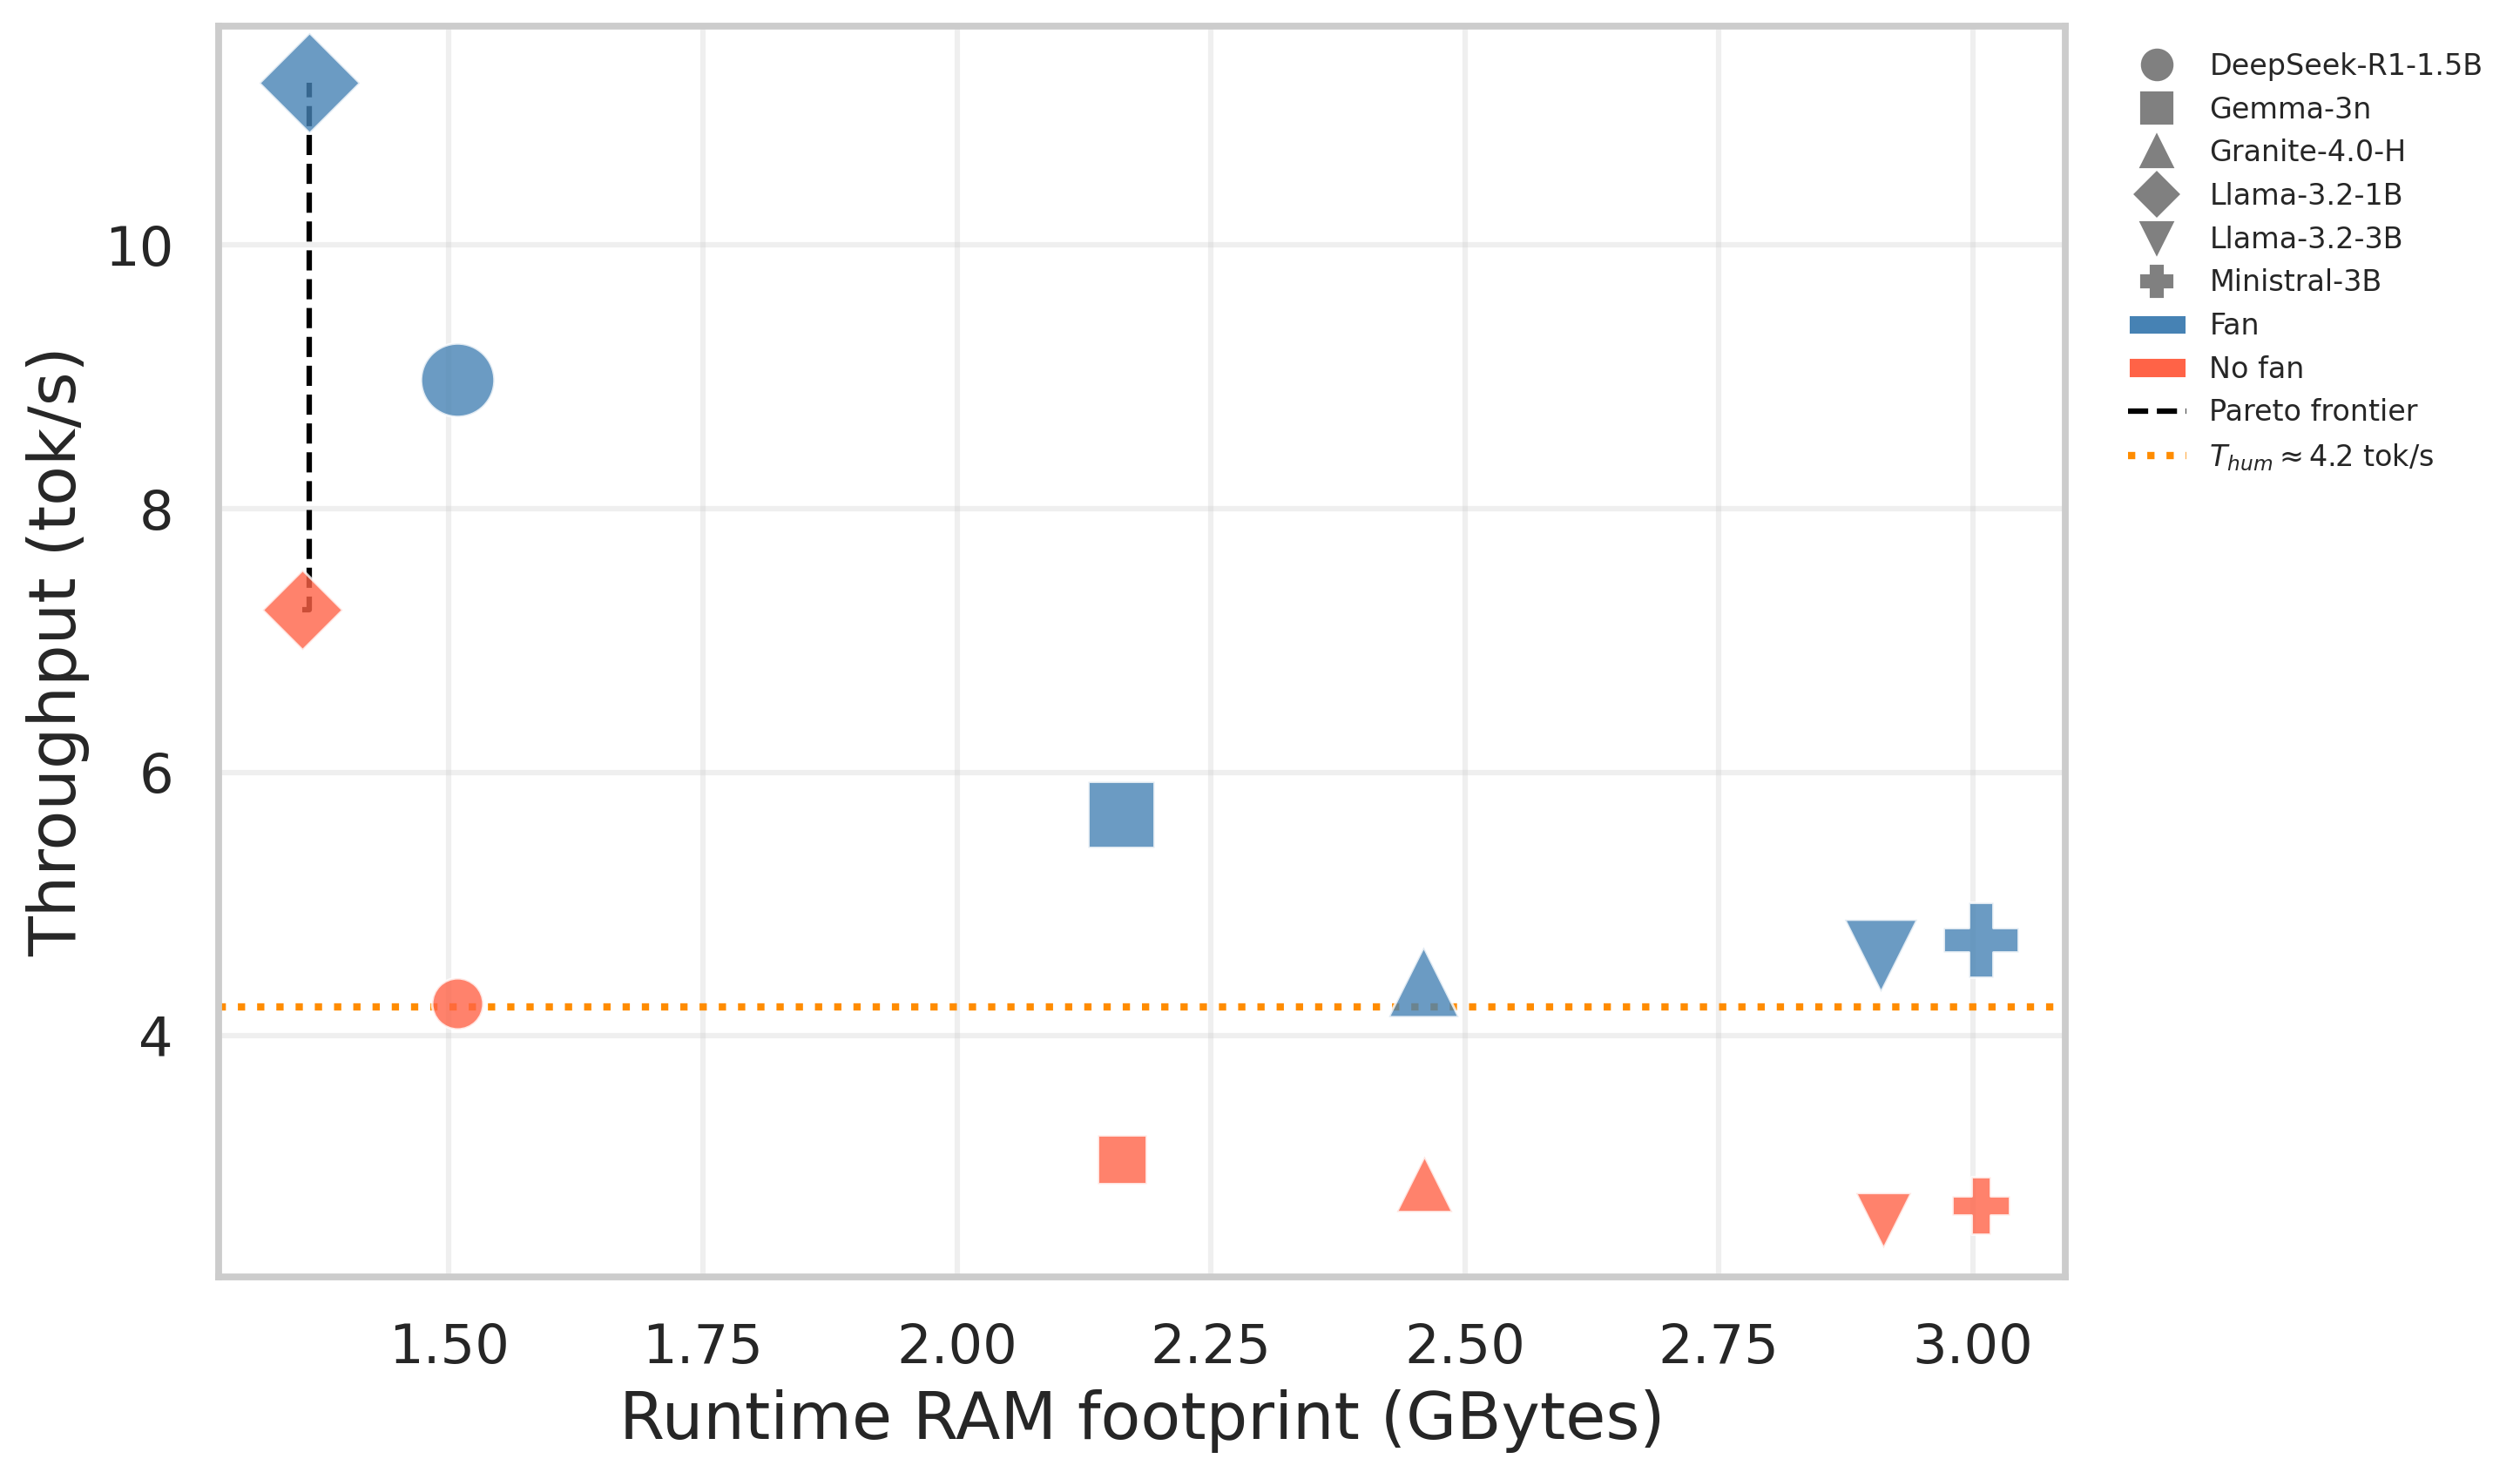
\includegraphics[width=\linewidth]{figures/e0_pareto.png}
\caption{Pareto frontier in the throughput (tok/s) versus RAM-footprint (GBytes)
plane for series E0, under active cooling (blue) and natural convection
(red). Marker size is proportional to $\mathrm{FoM}_{\mathrm{full}}$; the
dotted horizontal line marks the mean usability threshold
$T_{\mathrm{hum}}$. Reference configuration.}
\label{fig:e0_pareto}
\end{figure}

\begin{figure}[t]
\centering
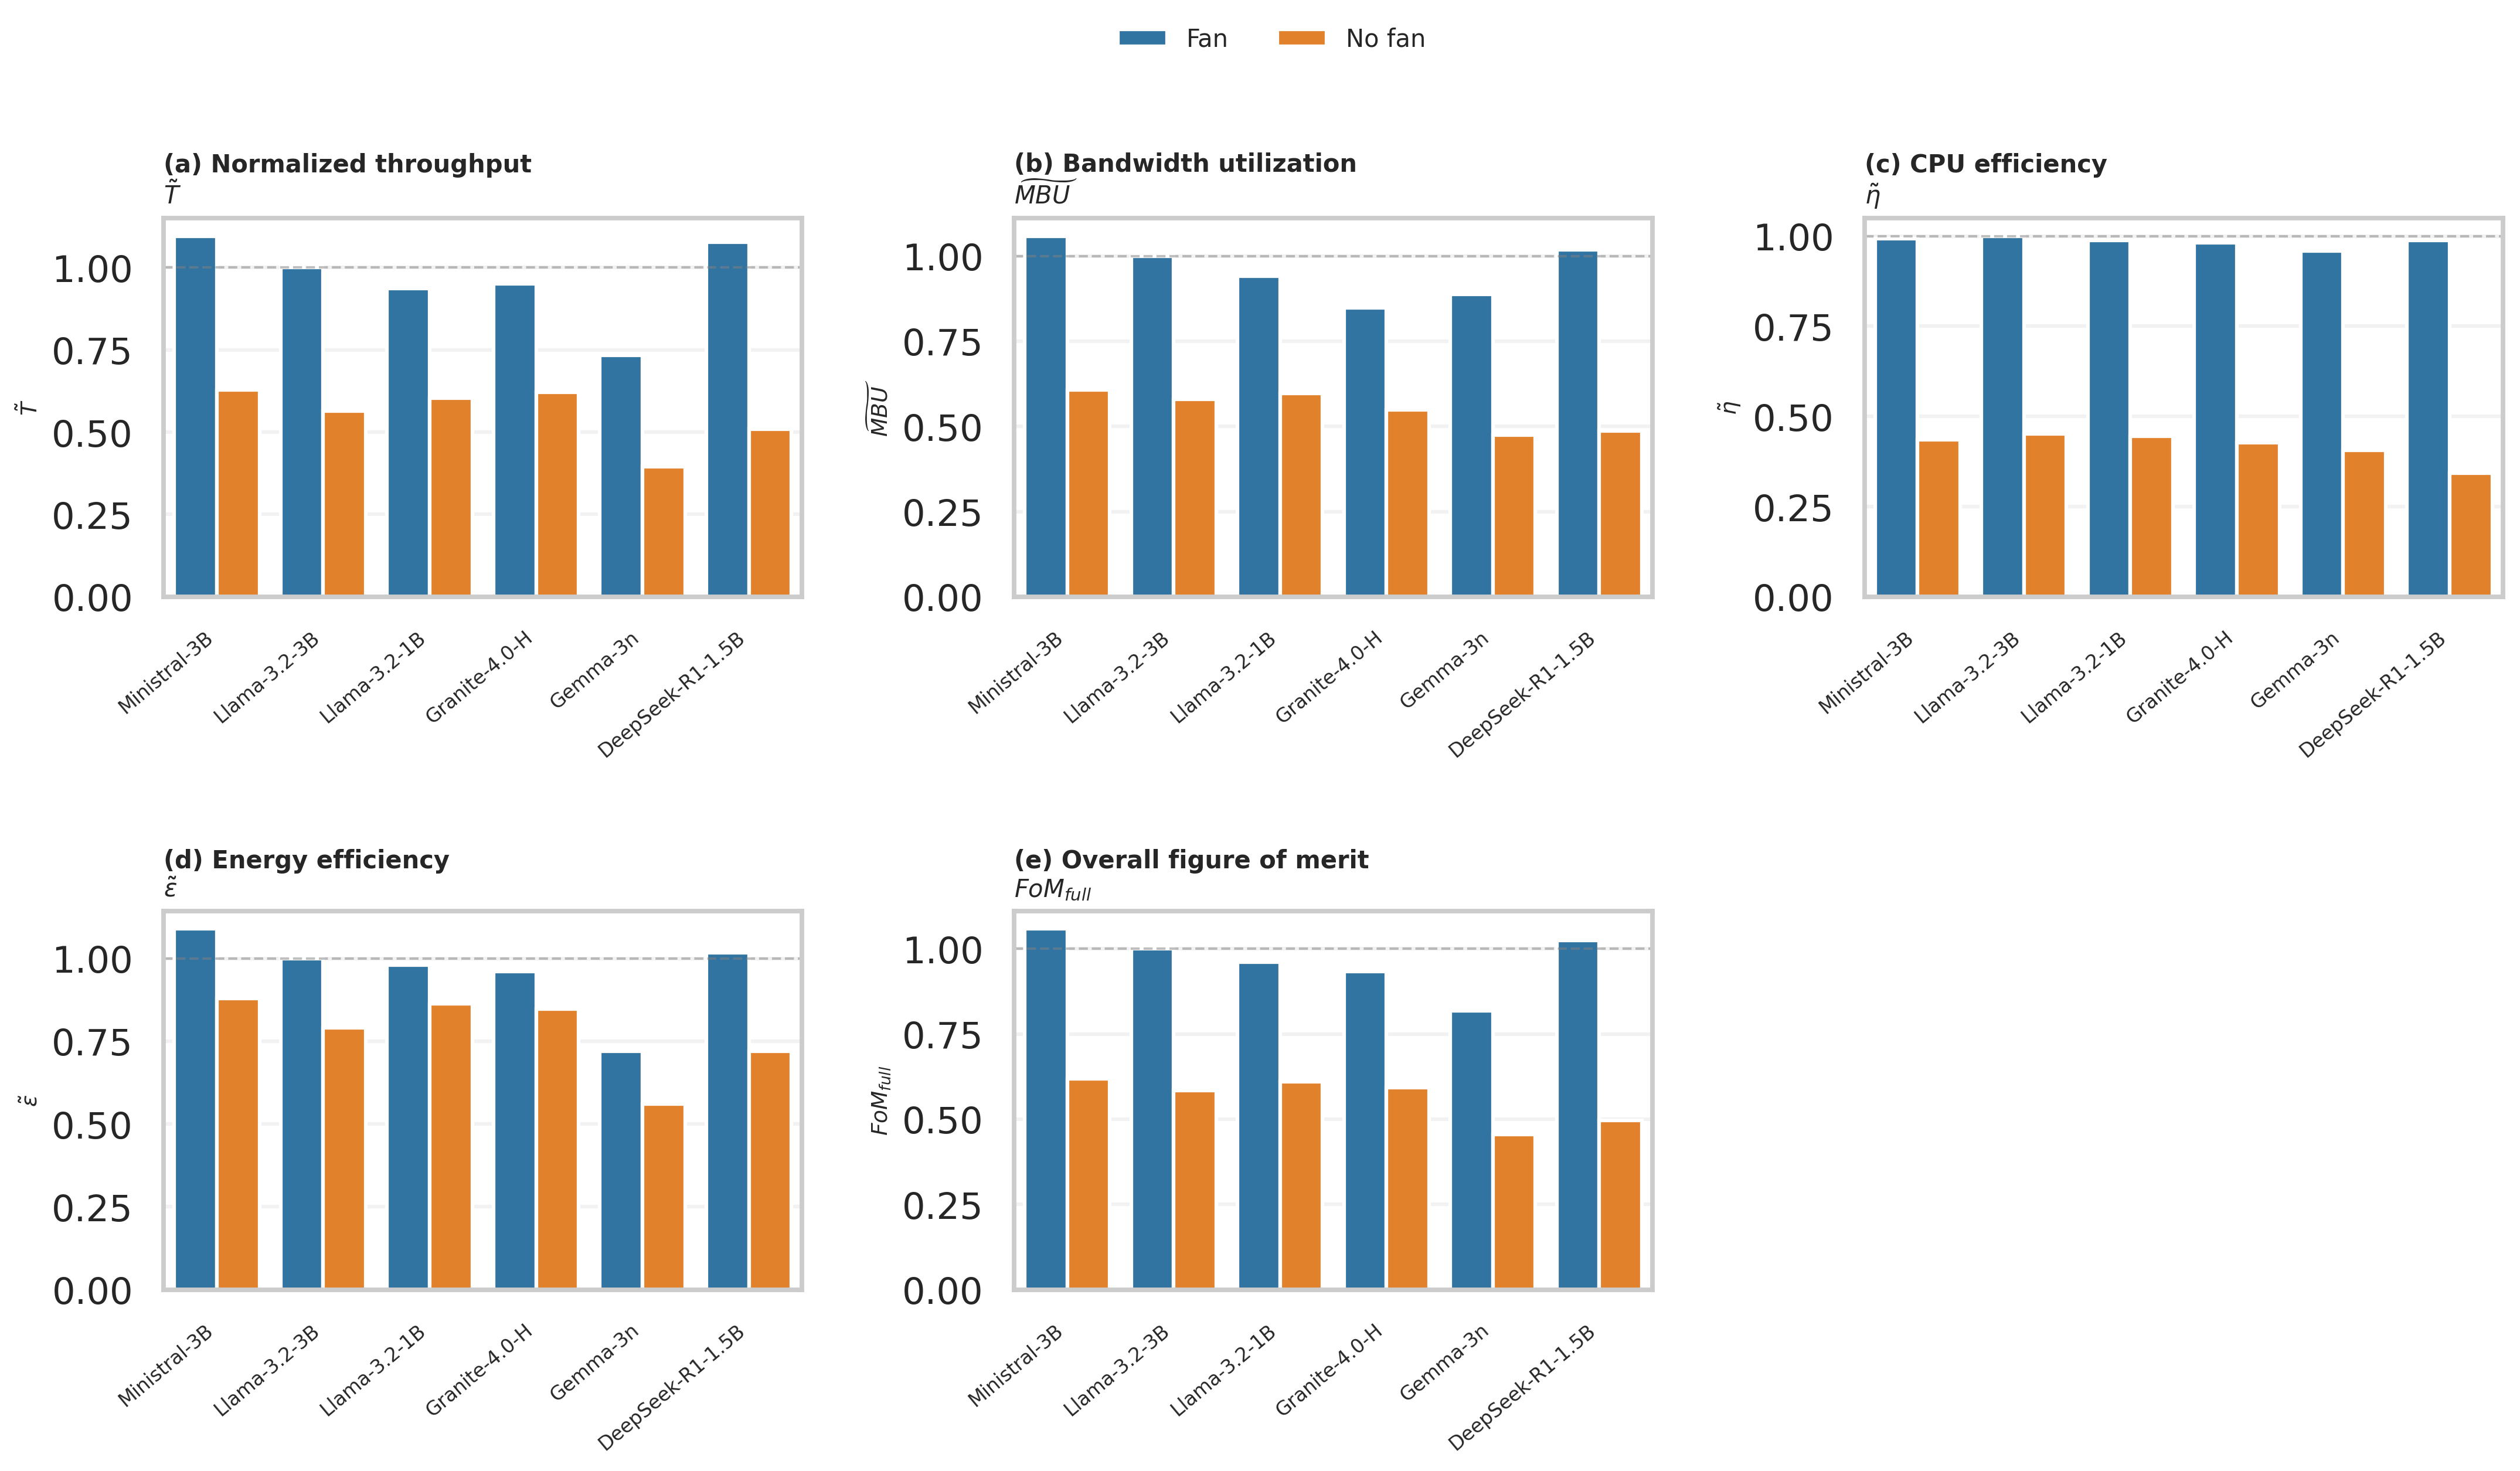
\includegraphics[width=\linewidth]{figures/e0_fom_decomposition.png}
\caption{Decomposition of $\mathrm{FoM}_{\mathrm{full}}$ into its four
normalized axes ($\tilde{T}$, $\widetilde{\mathrm{MBU}}$, $\tilde{\eta}$,
$\tilde{\varepsilon}$) per model and cooling condition, in the reference
configuration. Each axis is normalized with respect to Llama~3.2~3B under
active cooling.}
\label{fig:e0_fom}
\end{figure}

With active cooling, compute efficiency $\eta_{\mathrm{CPU}}$ is nearly
homogeneous across models (0.95--0.99) and therefore not a discriminating
axis; differentiation comes from corrected bandwidth utilization and weighted
energy efficiency (Figure~\ref{fig:e0_fom}). The platform operates
memory-bound during decoding, with $\mathrm{MBU}_{\mathrm{corr}}$ between 53
and 66\%.

\begin{figure}[t]
\centering
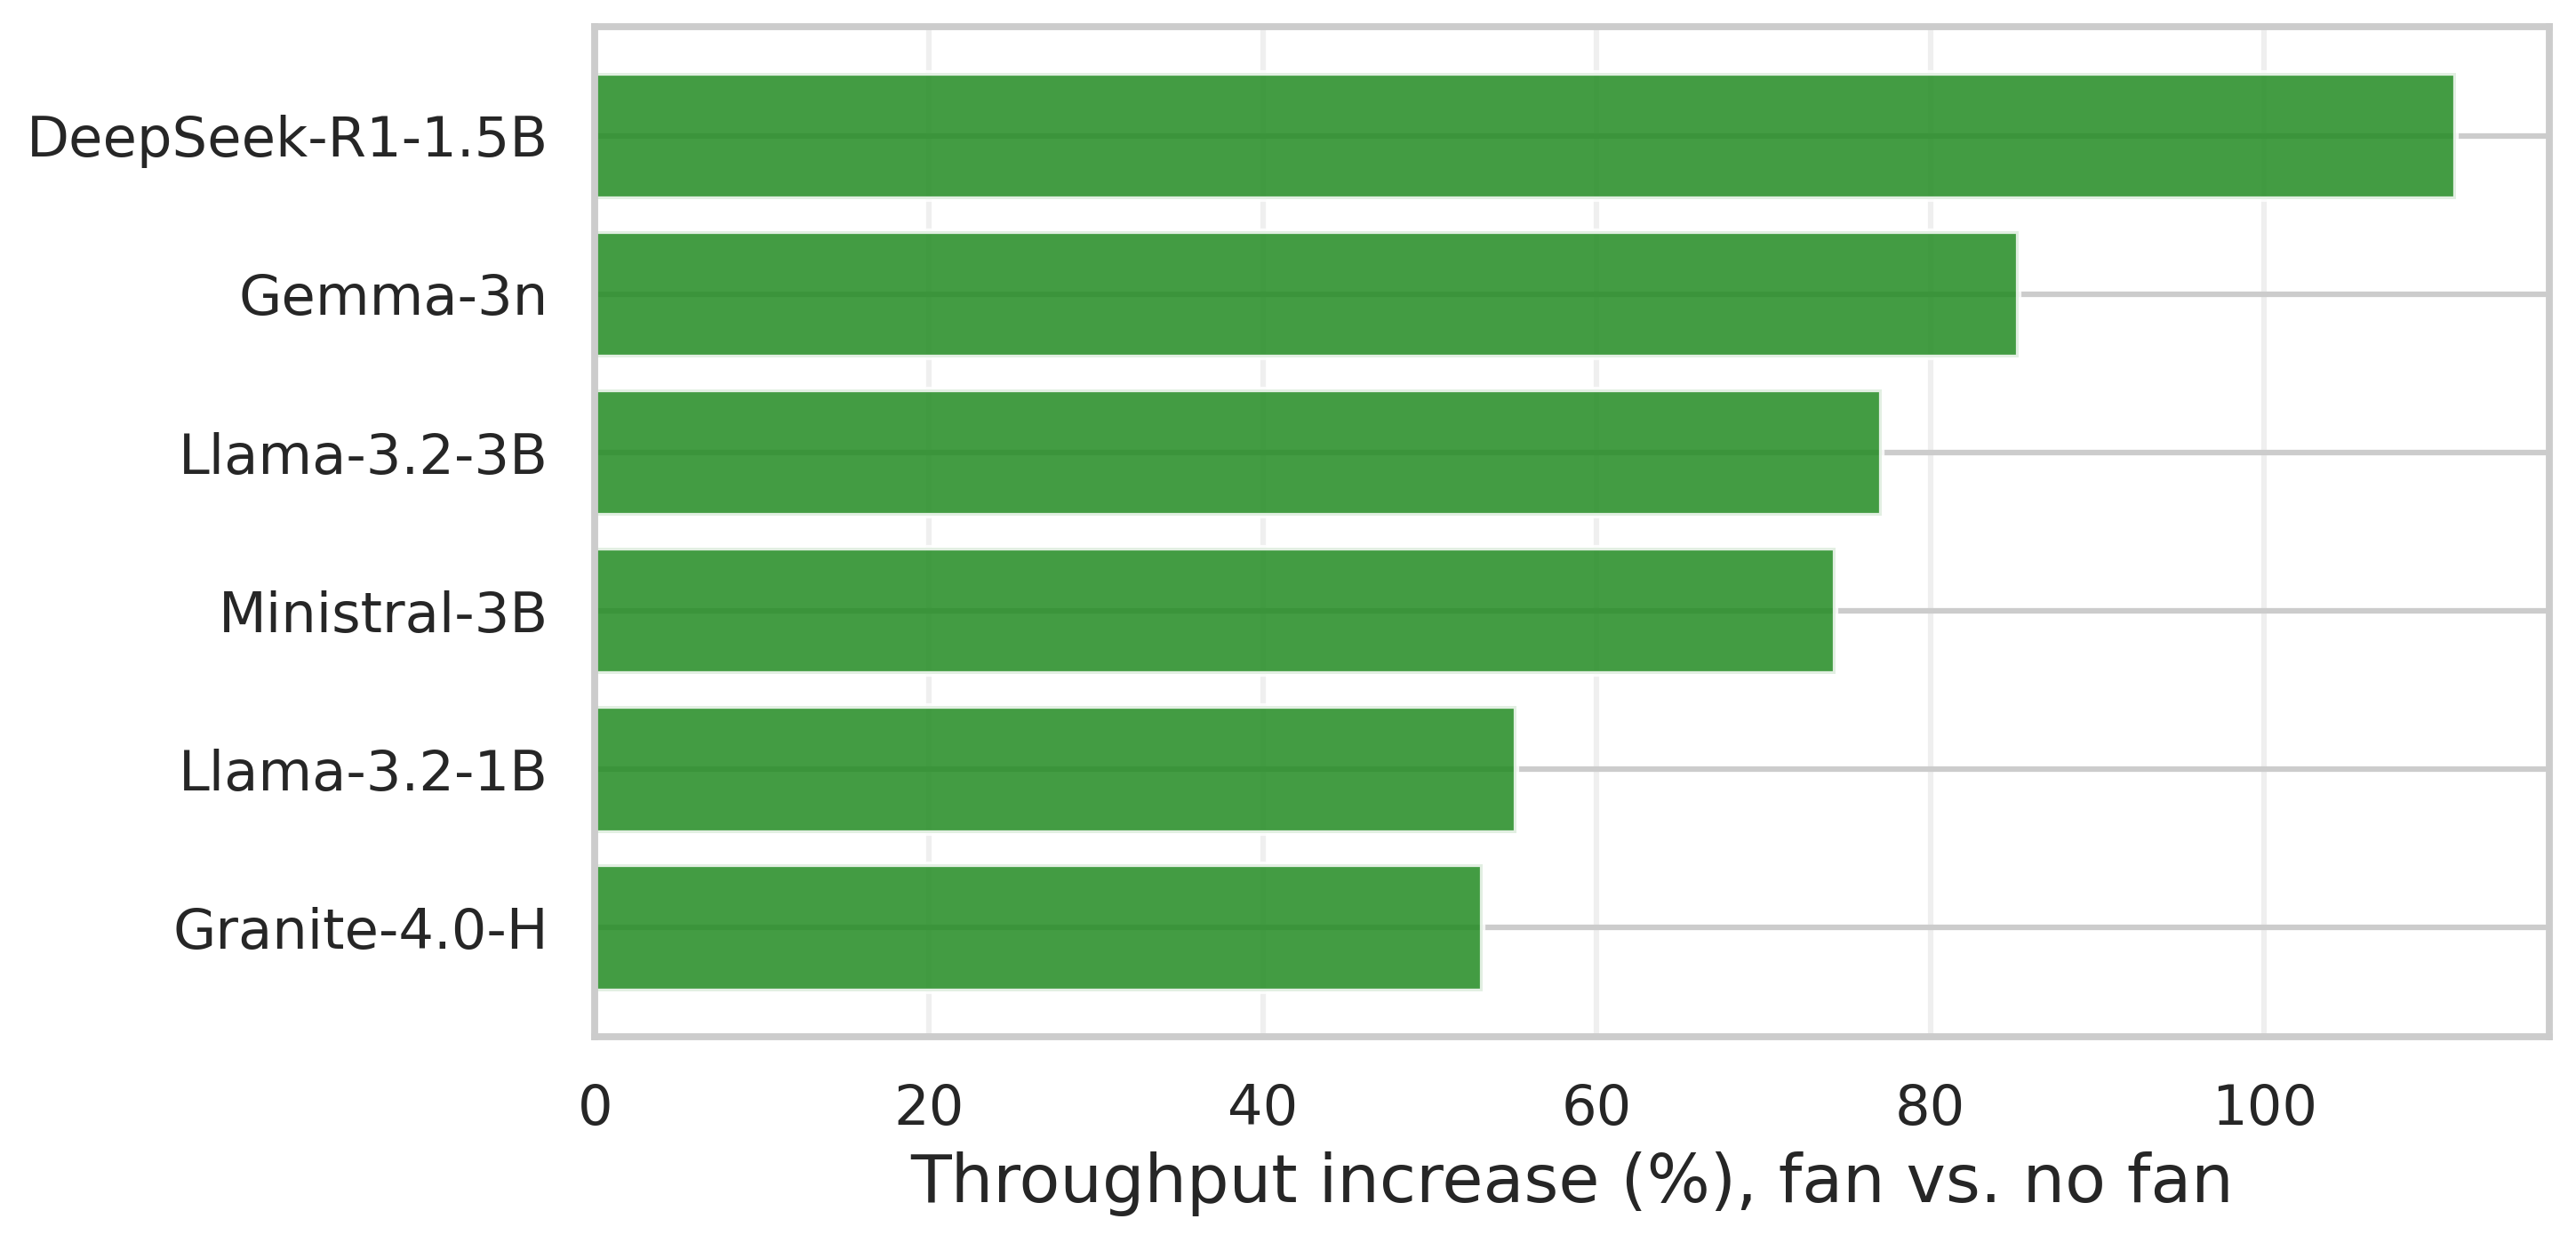
\includegraphics[width=\linewidth]{figures/e0_cooling_impact.png}
\caption{Percentage throughput increase when enabling active cooling (fan
vs.\ no fan) per model, in the reference configuration.}
\label{fig:e0_cooling}
\end{figure}

The effect of cooling is substantial and uneven
(Figure~\ref{fig:e0_cooling}). DeepSeek-R1~1.5B is the most sensitive, with a
111.5\% throughput increase when the fan is enabled, versus 55.2\% for
Llama~3.2~1B. The decisive integration result is the change of usability
state: without the fan, four of the six models (Ministral, Granite,
Llama~3.2~3B, Gemma~3n) fall below $T_{\mathrm{hum}}$ and cease to be
interactively usable. The collapse of $\eta_{\mathrm{CPU}}$ under natural
convection (from ${\approx}0.97$ to ${\approx}0.40$) confirms that the cause
is thermal throttling rather than any intrinsic model limitation. Active
cooling is therefore an enabling requirement, not a marginal optimization.

\begin{figure}[t]
\centering
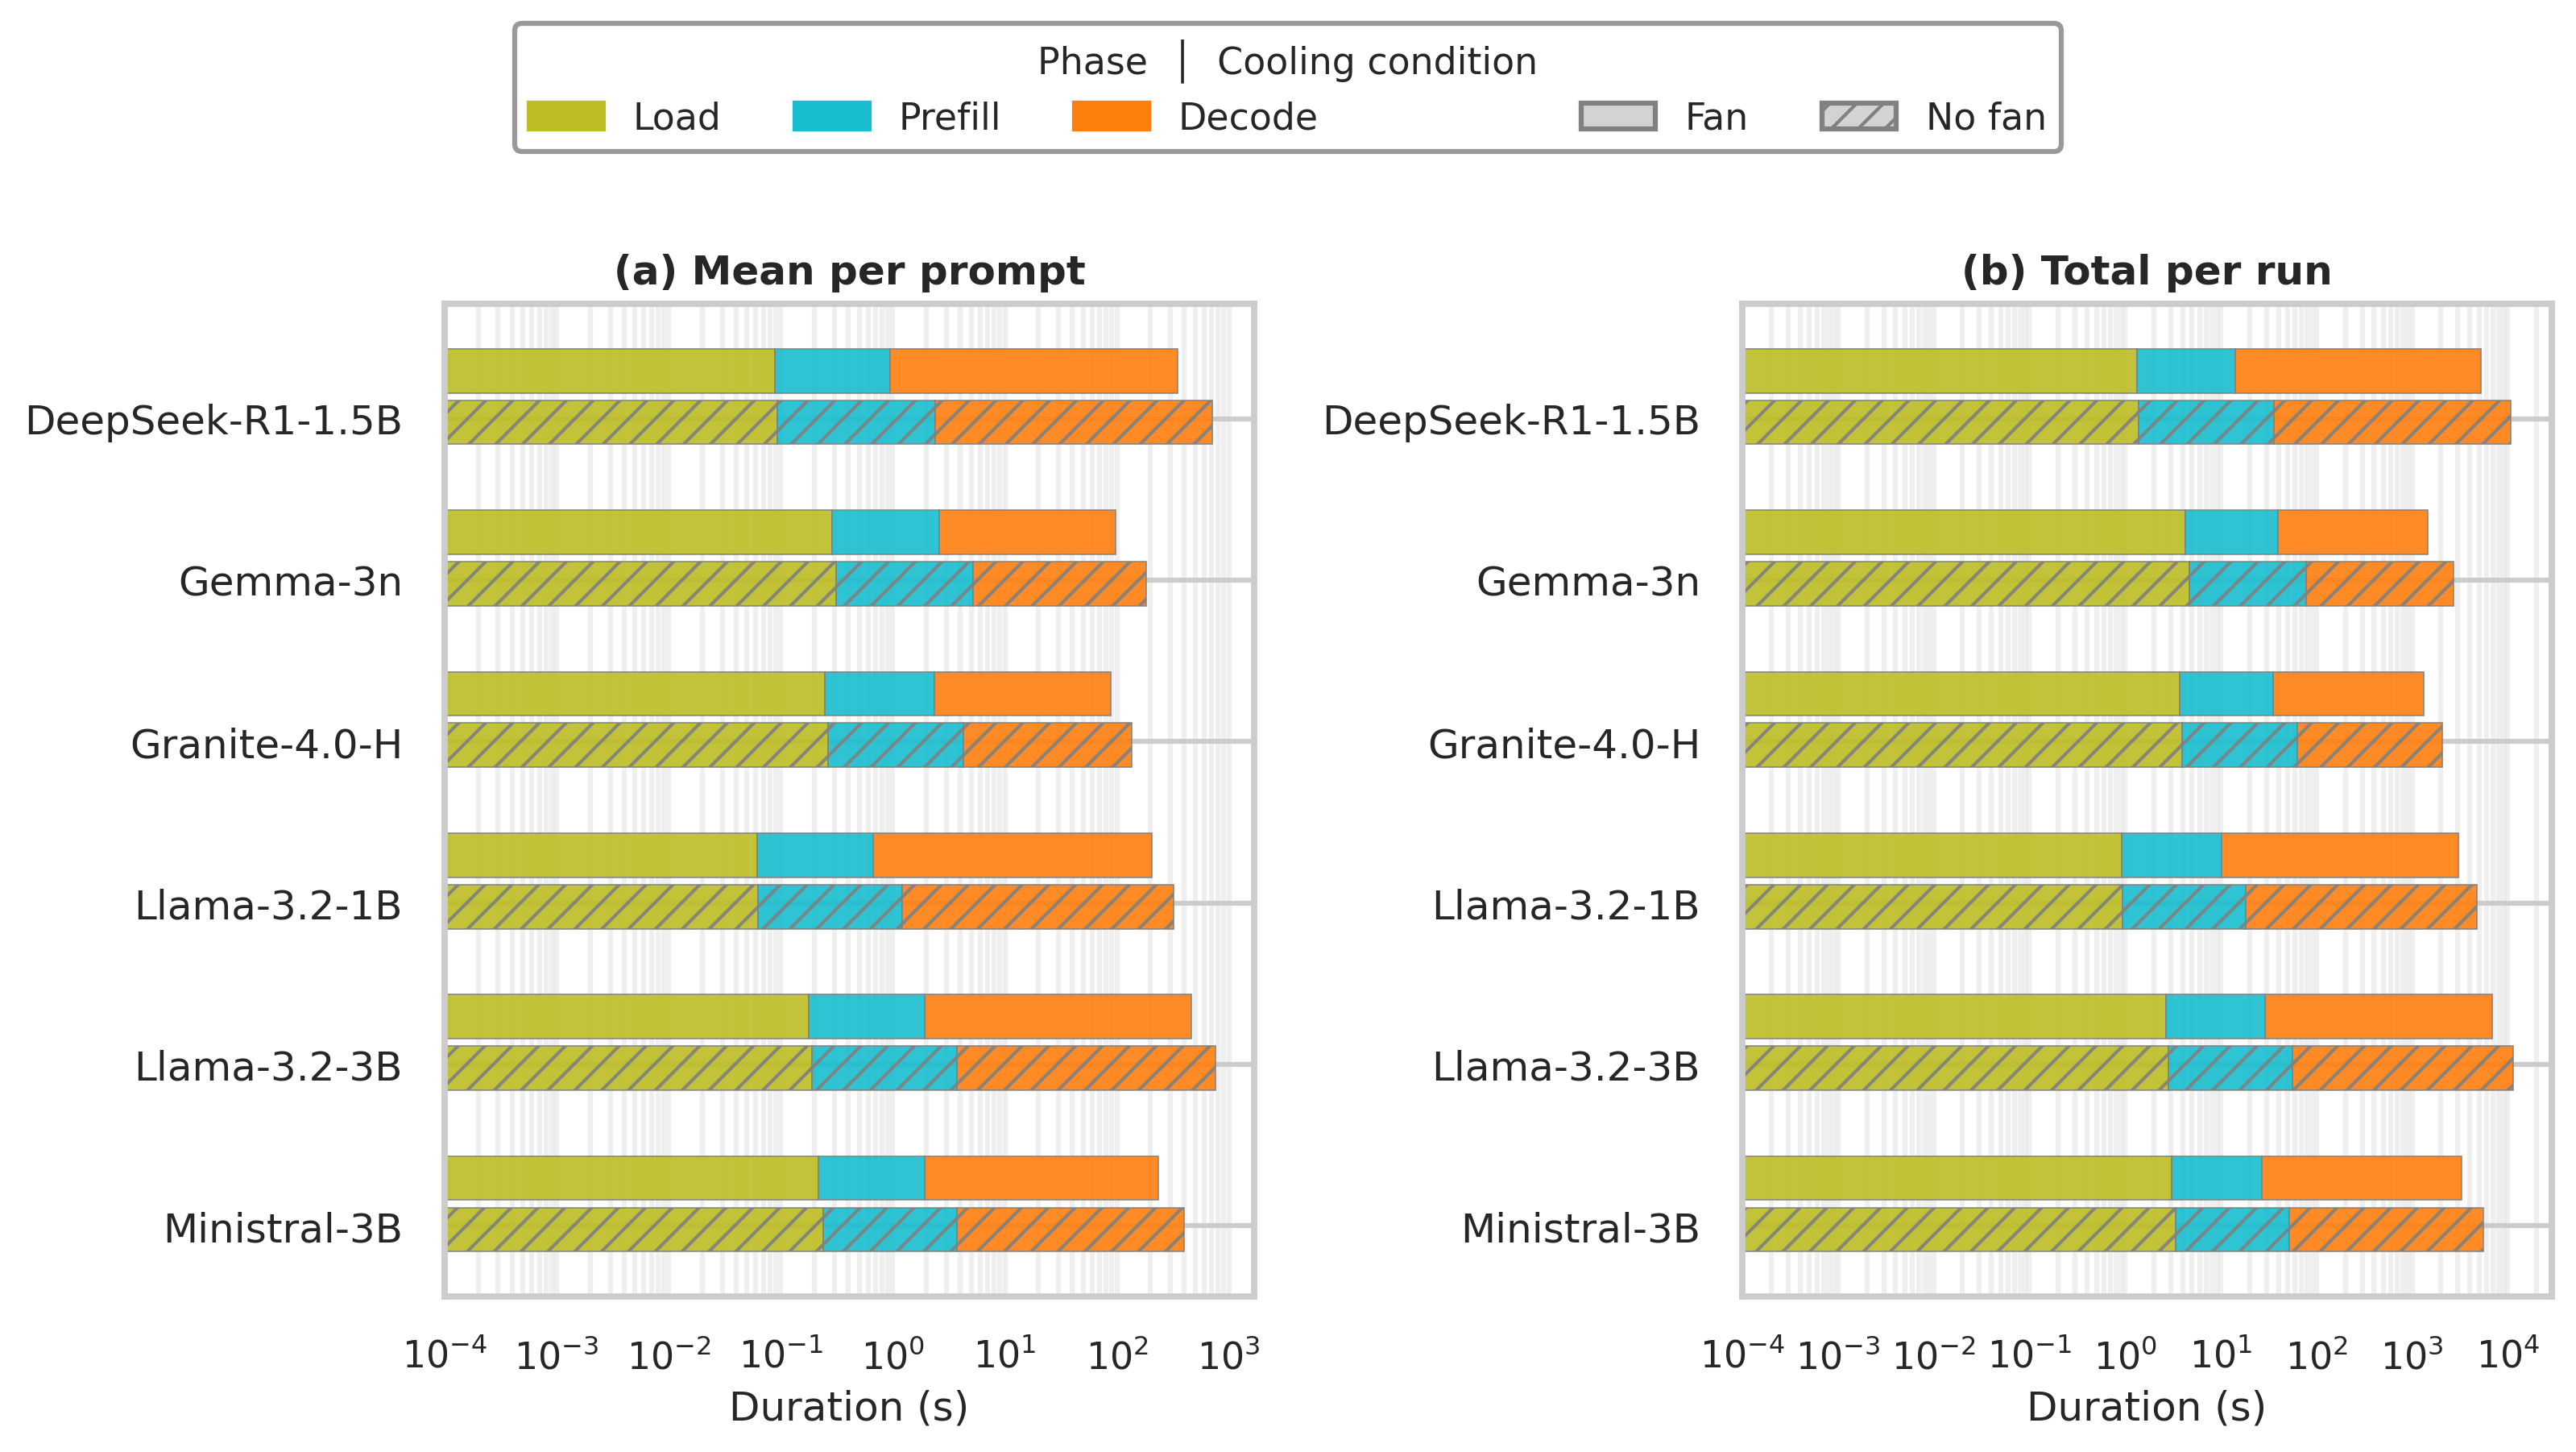
\includegraphics[width=\linewidth]{figures/e0_phase_breakdown.png}
\caption{Per-phase duration breakdown (load, prefill, decode) per model and
cooling condition in the reference configuration, on a logarithmic time axis:
(a)~mean per prompt and (b)~total per run. Solid bars correspond to active
cooling and hatched bars to natural convection. Note that the logarithmic
axis compresses the decode segment, which nevertheless accounts for
96.9--99.7\% of the total inference time across all configurations.}
\label{fig:e0_phases}
\end{figure}

Finally, the per-phase breakdown (Figure~\ref{fig:e0_phases}) shows that
decoding concentrates virtually the entire inference cost: model loading is
negligible in steady operation (0.06--0.29~s per prompt, supporting a
keep-resident strategy), prefill accounts for a small and stable fraction
(0.6--2.3~s per prompt), and decoding dominates (85--460~s per prompt, the
maximum corresponding to Llama~3.2~3B, the largest model of the set). All
per-phase values are means over prompts; since these distributions are
strongly right-skewed, the top of the ranking depends on the statistic used
(by median, the highest decode cost is that of DeepSeek-R1, 496~s versus
133~s for Llama~3.2~3B: the reasoning traces of the former make nearly every
response long, whereas the mean of the latter is driven by four out of fifteen
prompts above 1300~s). Given that decoding dominates, any
thermally induced frequency reduction translates proportionally into global
throughput loss, which explains the four models that become out of the
usability range under natural convection conditions (no fan).

\subsection{E1: Quantization}\label{sec:results_e1}

In series E1, we evaluated the effect of the quantization level, expressed in bits
per weight (bpw), across five GGUF levels per model (plus BF16 for
Llama~3.2~1B, the only model whose full-precision footprint fits the
platform), holding the rest of the reference configuration fixed (RQ2).
Generative quality was evaluated with PerplexitySystem on
WikiText-2~\cite{merity2016pointer} ($\mathrm{PPL}_{\mathrm{wk}}$); the DeepSeek-R1-1.5B runs in Q4\_0 and Q8\_0
were excluded from all analyses of the series due to model collapse
(generation of empty or incoherent sequences). Table~\ref{tab:e1} reports the results.

\begin{table}[!tp]
\centering
\caption{Inference, energy-efficiency, and quality metrics per model and
quantization level (series E1). $\mathrm{PPL}_{\mathrm{wk}}$ is computed over
the first 15\,000 tokens of WikiText-2~\cite{merity2016pointer} (context
512, teacher forcing);
standard error between chunks in parentheses. MBU is the corrected
memory-bandwidth utilization defined in Eq.~\eqref{eq:mbu_corr}. Bold: best
$\mathrm{FoM}_{\mathrm{full}}$ per model. $\dag$~DeepSeek-R1-1.5B Q4\_0 and
Q8\_0 excluded due to model collapse. \ding{55}: non-interactive
configuration ($T<T_{\mathrm{hum}}$).}
\label{tab:e1}
\renewcommand{\arraystretch}{1.02}
\setlength{\tabcolsep}{4.5pt}
\footnotesize
\begin{tabular}{@{}llrrrrrrlrc@{}}
\toprule
\textbf{Quant.} & \textbf{BPW} &
\textbf{RAM} & \textbf{$T$} & \textbf{$T_{\mathrm{hum}}$} &
\textbf{TTFT} & \textbf{$\varepsilon$} &
\textbf{MBU\textsubscript{corr}} & \textbf{PPL\textsubscript{wk}} &
\textbf{FoM\textsubscript{full}} & \textbf{Us.} \\
& & \textbf{(GByte)} & \textbf{(tok/s)} & \textbf{(tok/s)} & \textbf{(ms)} & \textbf{(tok/J)} & \textbf{(\%)} & & & \\
\midrule
\multicolumn{11}{@{}l}{\textit{DeepSeek-R1-1.5B}$^{\dag}$} \\[1pt]
Q5\_K\_M & 5.8 & 1.65 &  8.7 & 3.81 & 1076 & 1.131 & 69.9 & 41.75 (1.28) & 1.017 & \ding{51} \\
Q4\_K\_M & 5.0 & 1.51 &  8.9 & 3.69 &  952 & 1.257 & 63.2 & 43.66 (1.34) & 1.026 & \ding{51} \\
Q3\_K\_M & 4.2 & 0.98 & 10.0 & 3.62 & 1810 & 1.316 & 59.6 & 46.06 (1.44) & \textbf{1.051} & \ding{51} \\
\midrule
\multicolumn{11}{@{}l}{\textit{Llama-3.2-1B}} \\[1pt]
BF16     & 16.1 & 0.56 &  1.6 & 4.08 & 21514 & 0.218 & 24.6 & 14.69 (0.34) & 0.286 & \ding{55} \\
Q8\_0    &  8.6 & 1.87 &  7.6 & 3.86 &   951 & 1.211 & 63.7 & 14.71 (0.34) & 0.818 & \ding{51} \\
Q5\_K\_M &  5.9 & 1.46 & 11.2 & 3.83 &   752 & 1.543 & 66.7 & 14.86 (0.34) & 0.964 & \ding{51} \\
Q4\_K\_M &  5.2 & 1.36 & 11.7 & 4.01 &   674 & 1.809 & 60.7 & 15.23 (0.35) & \textbf{0.992} & \ding{51} \\
Q4\_0    &  5.0 & 1.32 & 11.2 & 3.92 &   458 & 1.805 & 56.2 & 17.27 (0.41) & 0.964 & \ding{51} \\
Q3\_K\_M &  4.5 & 0.97 & 11.4 & 3.90 &  1305 & 1.616 & 51.2 & 17.17 (0.40) & 0.919 & \ding{51} \\
\midrule
\multicolumn{11}{@{}l}{\textit{Llama-3.2-3B}} \\[1pt]
Q8\_0    & 8.5 & 4.34 & 3.2 & 4.05 & 2830 & 0.487 & 71.5 & 10.89 (0.24) & 0.869 & \ding{55} \\
Q5\_K\_M & 5.8 & 3.21 & 4.3 & 4.03 & 2194 & 0.582 & 67.7 & 10.98 (0.24) & 0.966 & \ding{51} \\
Q4\_K\_M & 5.0 & 2.91 & 4.6 & 4.25 & 1936 & 0.673 & 62.4 & 11.24 (0.25) & 1.000 & \ding{51} \\
Q4\_0    & 4.8 & 2.81 & 5.0 & 4.04 & 1197 & 0.766 & 64.1 & 11.52 (0.26) & 1.060 & \ding{51} \\
Q3\_K\_M & 4.2 & 1.82 & 5.5 & 3.92 & 3562 & 0.751 & 62.6 & 12.07 (0.27) & \textbf{1.074} & \ding{51} \\
\midrule
\multicolumn{11}{@{}l}{\textit{Gemma-3n (2B active)}} \\[1pt]
Q8\_0    & 8.6 & 3.18 & 3.8 & 4.58 & 3309 & 0.585 & 51.3 & 35.54 (1.27) & 0.670 & \ding{55} \\
Q5\_K\_M & 6.3 & 2.36 & 5.2 & 4.43 & 2933 & 0.684 & 53.2 & 33.83 (1.19) & 0.758 & \ding{51} \\
Q4\_K\_M & 5.9 & 2.16 & 5.6 & 4.45 & 2693 & 0.808 & 55.0 & 36.06 (1.28) & 0.814 & \ding{51} \\
Q4\_0    & 5.8 & 2.10 & 5.7 & 4.36 & 2219 & 0.851 & 55.1 & 37.78 (1.33) & 0.832 & \ding{51} \\
Q3\_K\_M & 5.5 & 1.43 & 6.2 & 4.35 & 3864 & 0.830 & 57.0 & 33.00 (1.14) & \textbf{0.850} & \ding{51} \\
\midrule
\multicolumn{11}{@{}l}{\textit{Granite-4.0-H-Micro}} \\[1pt]
Q8\_0    & 8.5 & 3.92 & 2.8 & 4.05 & 3480 & 0.439 & 58.1 &  9.96 (0.24) & 0.776 & \ding{55} \\
Q5\_K\_M & 5.7 & 2.79 & 3.9 & 3.98 & 2747 & 0.515 & 54.7 & 10.10 (0.24) & 0.863 & \ding{55} \\
Q4\_K\_M & 4.9 & 2.46 & 4.4 & 3.99 & 2365 & 0.647 & 52.9 & 10.39 (0.25) & 0.932 & \ding{51} \\
Q4\_0    & 4.7 & 2.37 & 4.5 & 4.04 & 1616 & 0.705 & 52.2 & 10.08 (0.23) & 0.956 & \ding{51} \\
Q3\_K\_M & 3.9 & 1.09 & 5.2 & 4.22 & 4532 & 0.673 & 50.4 & 11.88 (0.29) & \textbf{0.968} & \ding{51} \\
\midrule
\multicolumn{11}{@{}l}{\textit{Ministral-3B}} \\[1pt]
Q8\_0    & 8.5 & 4.51 & 3.0 & 4.51 & 3016 & 0.447 & 69.7 &  8.43 (0.17) & 0.858 & \ding{55} \\
Q5\_K\_M & 5.8 & 3.33 & 4.2 & 4.59 & 2342 & 0.541 & 67.8 &  8.47 (0.17) & 0.971 & \ding{55} \\
Q4\_K\_M & 5.0 & 3.01 & 4.9 & 4.50 & 1874 & 0.701 & 71.2 &  8.57 (0.17) & 1.091 & \ding{51} \\
Q4\_0    & 4.8 & 2.90 & 5.1 & 4.65 & 1164 & 0.764 & 68.4 &  8.90 (0.18) & \textbf{1.118} & \ding{51} \\
Q3\_K\_M & 4.2 & 1.85 & 5.5 & 4.68 & 3630 & 0.697 & 67.0 &  9.13 (0.18) & 1.108 & \ding{51} \\
\bottomrule
\end{tabular}
\end{table}

The most relevant result is that aggressive quantization not only
reduces the memory footprint but \emph{improves} the FoM in every
model: $\mathrm{FoM}_{\mathrm{full}}$ grows monotonically from Q8\_0 towards
Q4 and Q3, peaking at Q4\_0 or Q3\_K\_M depending on the model. The cause is
twofold: a smaller footprint reduces per-token memory traffic---the binding
constraint on this memory-bound platform---, raising throughput and energy
efficiency $\varepsilon$ at the same time. Conversely, Q8\_0 falls
below the usability threshold in four of the six models, and BF16 sinks
Llama~3.2~1B to 1.6~tok/s (Figure~\ref{fig:e1_fom_bpw}): on a memory-bound
platform, excess precision is counterproductive.

\begin{figure}[t]
\centering
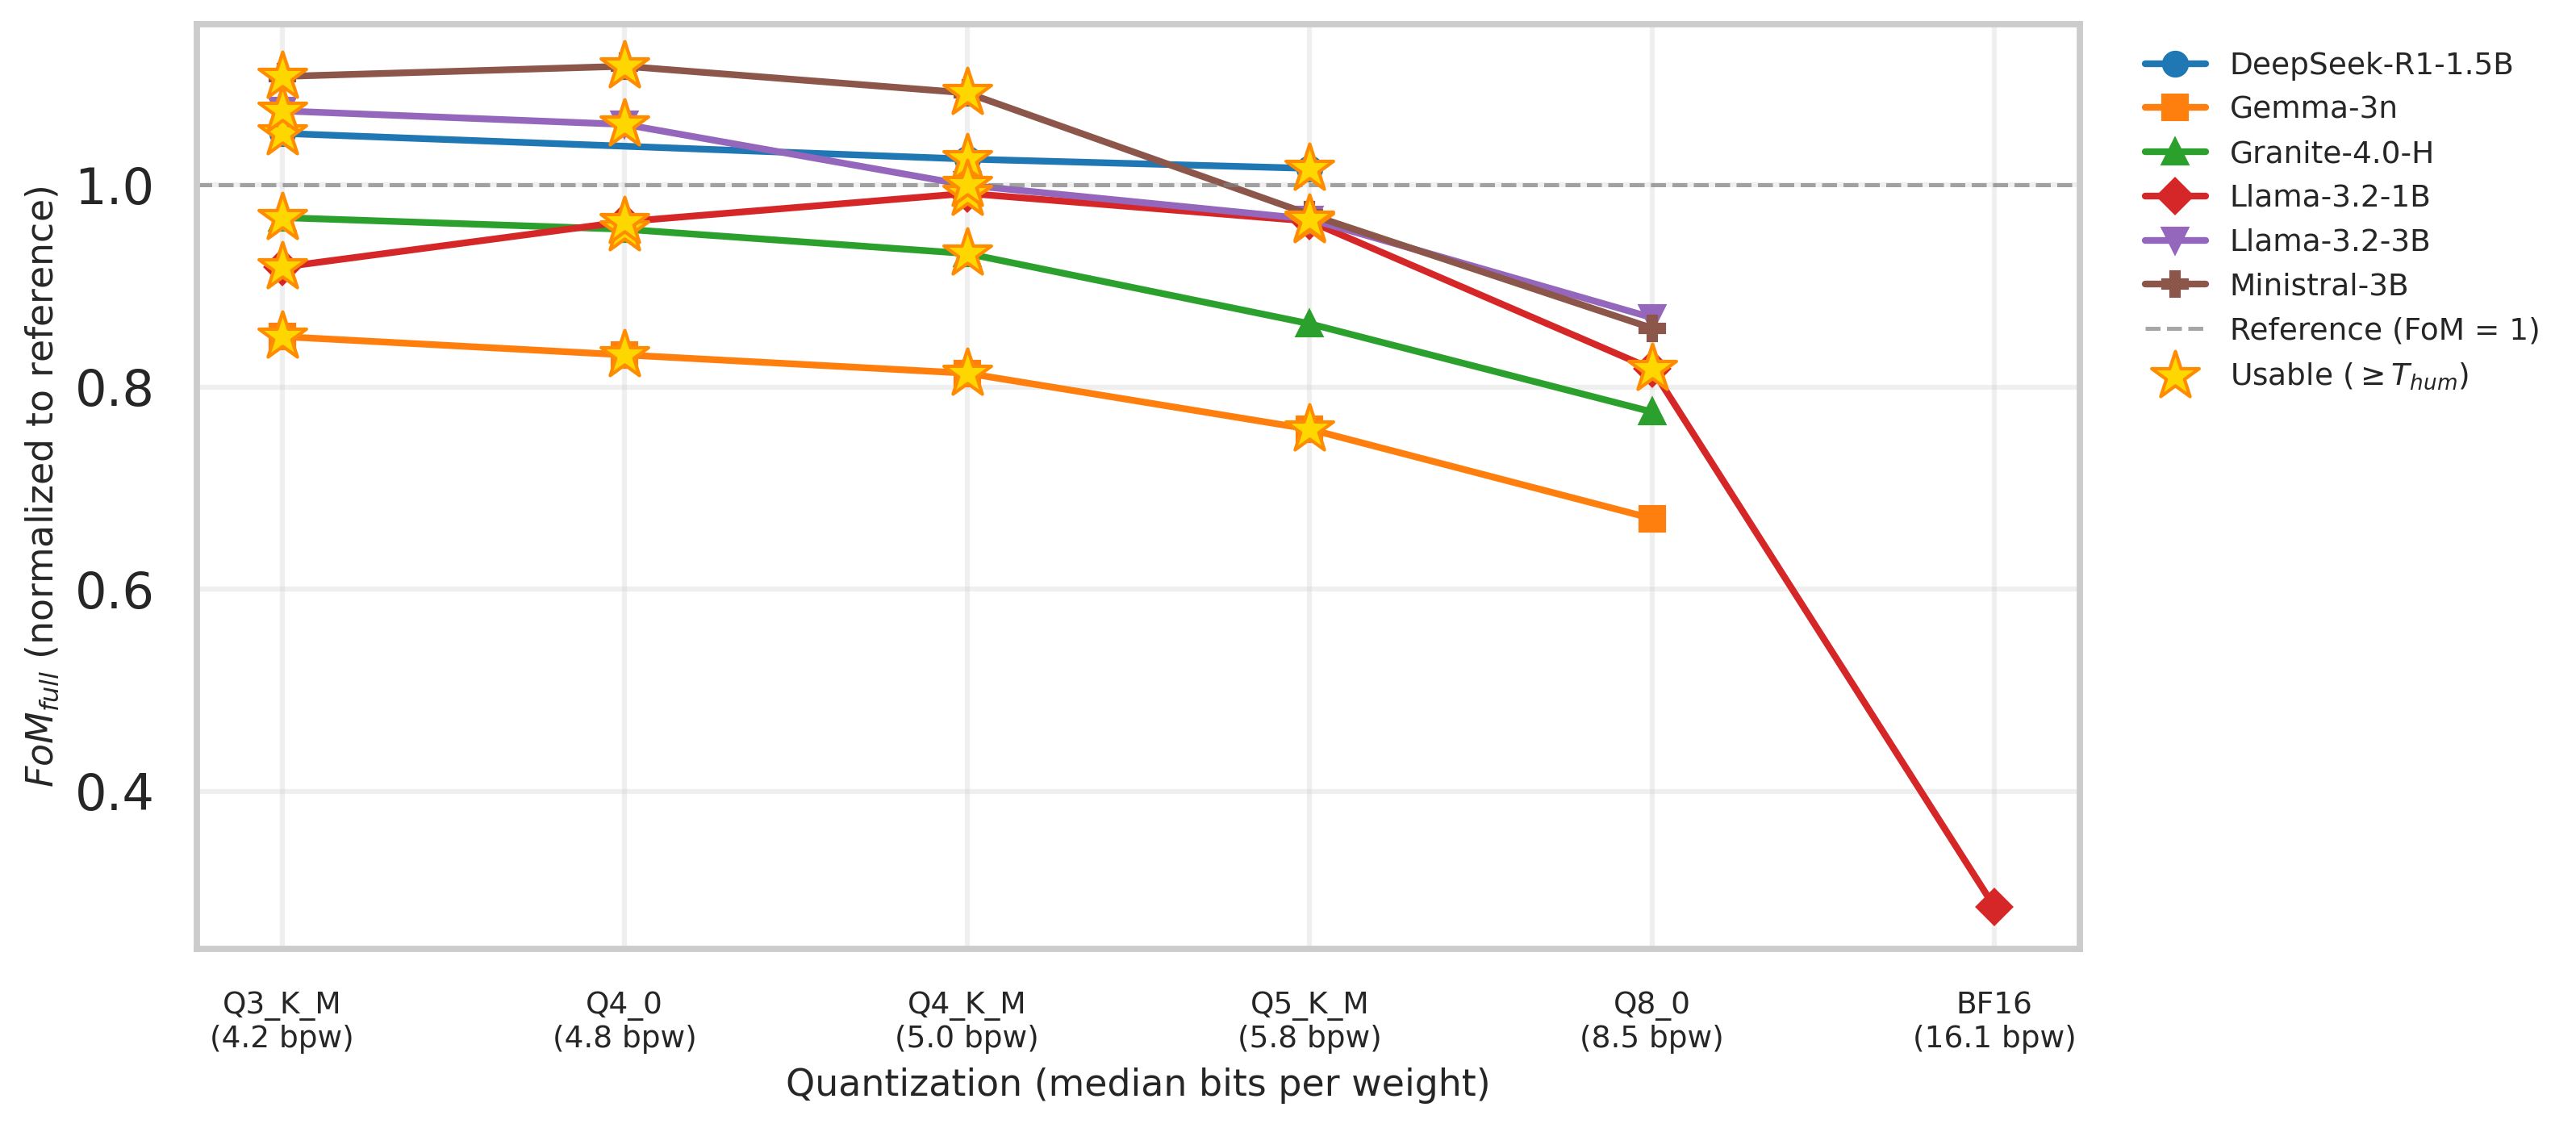
\includegraphics[width=0.85\linewidth]{figures/e1_fom_bpw.png}
\caption{$\mathrm{FoM}_{\mathrm{full}}$ as a function of bits per weight
(bpw), one line per model; precision decreases from left to right. The dashed
horizontal line marks the reference level ($\mathrm{FoM}=1$); stars mark
usable configurations ($T \geq T_{\mathrm{hum}}$, Table~\ref{tab:models}).
Reference configuration,
active cooling.}
\label{fig:e1_fom_bpw}
\end{figure}

\begin{figure}[t]
\centering
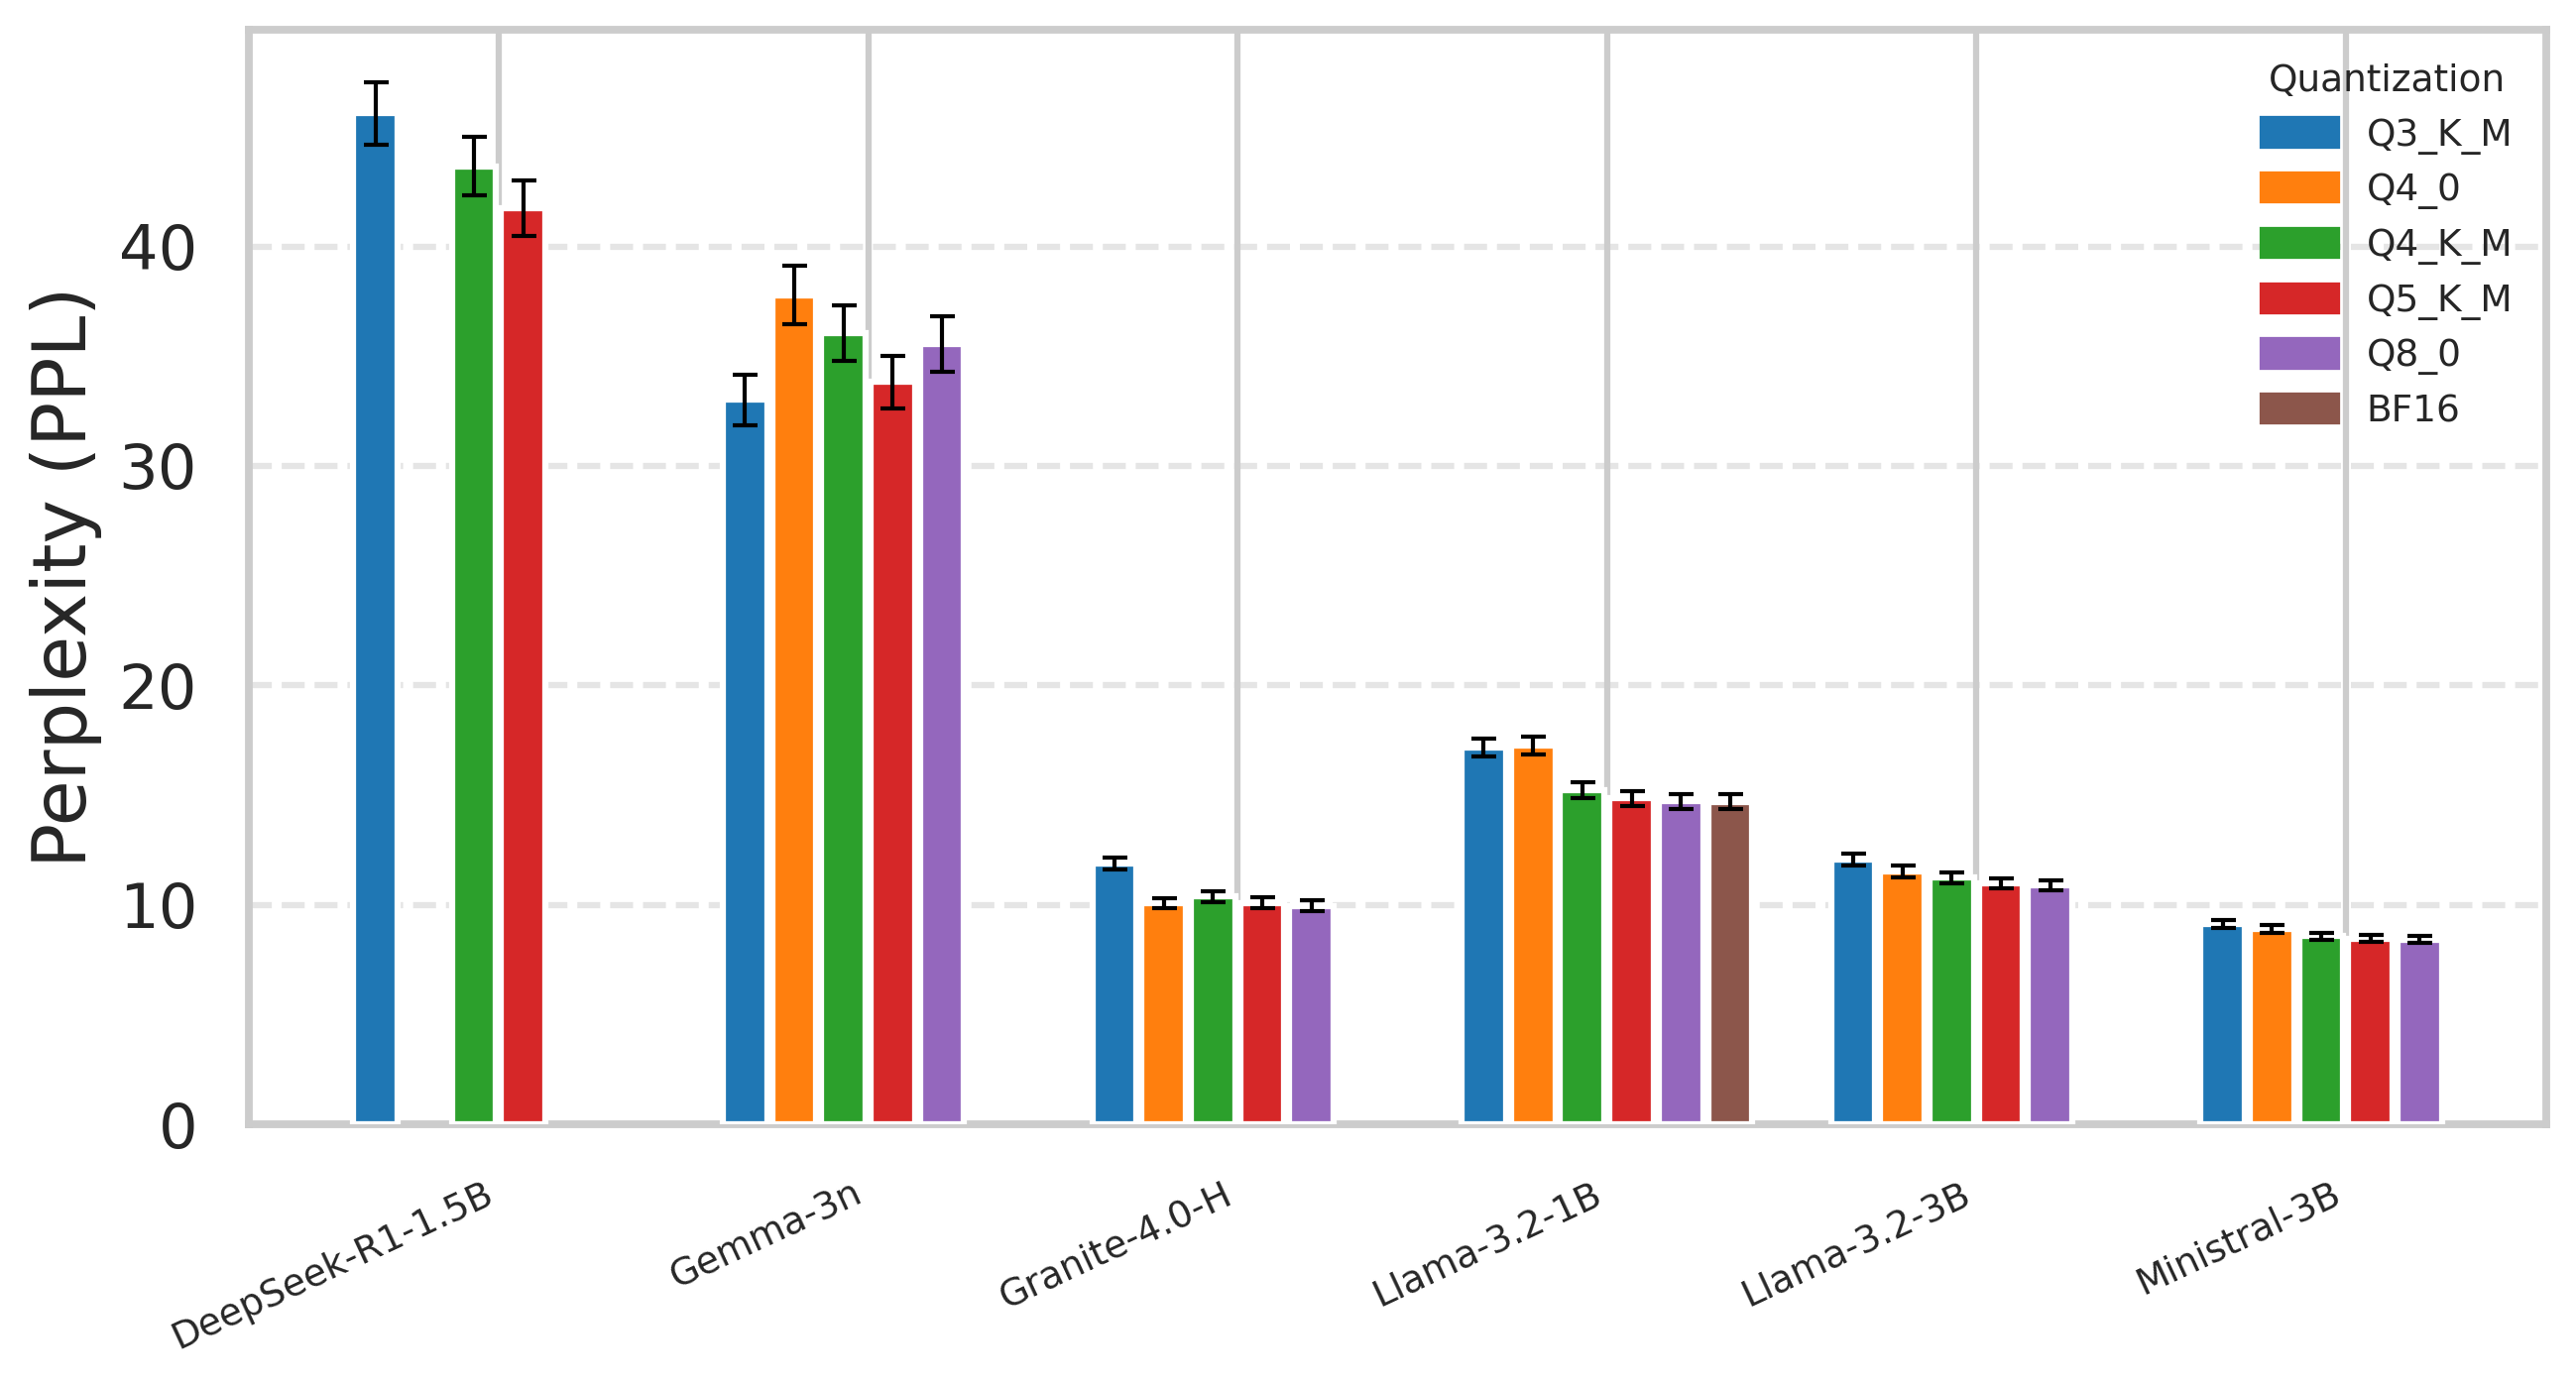
\includegraphics[width=0.88\linewidth]{figures/e1_perplexity.png}
\caption{WikiText-2~\cite{merity2016pointer} perplexity
($\mathrm{PPL}_{\mathrm{wk}}$, context 512,
teacher forcing) per model and quantization level. Error bands are the
standard error between chunks. Only K-quant levels are shown for
DeepSeek-R1-1.5B (Q4\_0 and Q8\_0 collapse; see text).}
\label{fig:e1_ppl}
\end{figure}

In the quality dimension (Figure~\ref{fig:e1_ppl}), the degradation from
Q8\_0 to Q4\_K\_M is below 5\% in all models (Ministral-3B: $+1.7\%$;
Llama-3.2-3B: $+3.2\%$; Llama-3.2-1B: $+3.5\%$; Granite: $+4.3\%$), and
Q5\_K\_M is virtually lossless ($<1.4\%$). Q3\_K\_M introduces appreciable
degradation (8--19\% depending on the model). Notably, Q4\_0, despite
sharing the bit level of Q4\_K\_M, degrades quality more in every model (up
to $+13.4\%$ in Llama-3.2-1B), while offering no systematic advantage in
throughput or energy; the choice between K and non-K families is therefore
decisive for quality though not for performance, making K-quants preferable
in all scenarios except under extreme load-latency constraints. These
results are consistent with Kurtic et al.~\cite{kurtic_give_2025} and
validate, in the edge-inference context, that 4-bit quantization preserves
generative quality within operationally acceptable margins. In summary,
Q4\_K\_M is the recommended default operating point---usable in all six
models with low TTFT and near-baseline quality---with Q4\_0 and Q3\_K\_M as
alternatives under stronger resource constraints (e.g., Llama-3.2-1B at Q3\_K\_M
runs in 0.97~GByte at 11.4~tok/s).

\subsection{E2: Context-Window Size}\label{sec:results_e2}

In series E2, we varied the context window across 512--5\,120~tokens (RQ3). Three
practical observations emerge. First, the RAM footprint grows smoothly and
predictably with context, reflecting the KV-cache cost: between $+2\%$
(Granite, whose fixed-size SSM state requires no growing KV cache) and
$+21\%$ (Llama~3.2~3B) over the full range, never exceeding 3.2~GByte---context
is not a memory-pressure factor against the platform's 8~GByte RAM. Second, TTFT
remains essentially flat: reserving a larger window does not increase
prefill cost while the prompt does not fill it. Third, throughput decreases
smoothly and monotonically with context
(Figure~\ref{fig:e2_throughput}), with losses up to 22\% in the models with
the highest bandwidth utilization (DeepSeek $-22\%$, Llama-3.2-1B $-18\%$):
the closer a model is to saturating memory bandwidth, the more sensitive it
is to the growing per-token KV-cache traffic. Gemma~3n and Granite, with MBU
below 55\%, are practically insensitive. No model crosses the usability
threshold within the range. The practical recommendation is to size the
context to the smallest value that covers the application's needs.

\begin{figure}[t]
\centering
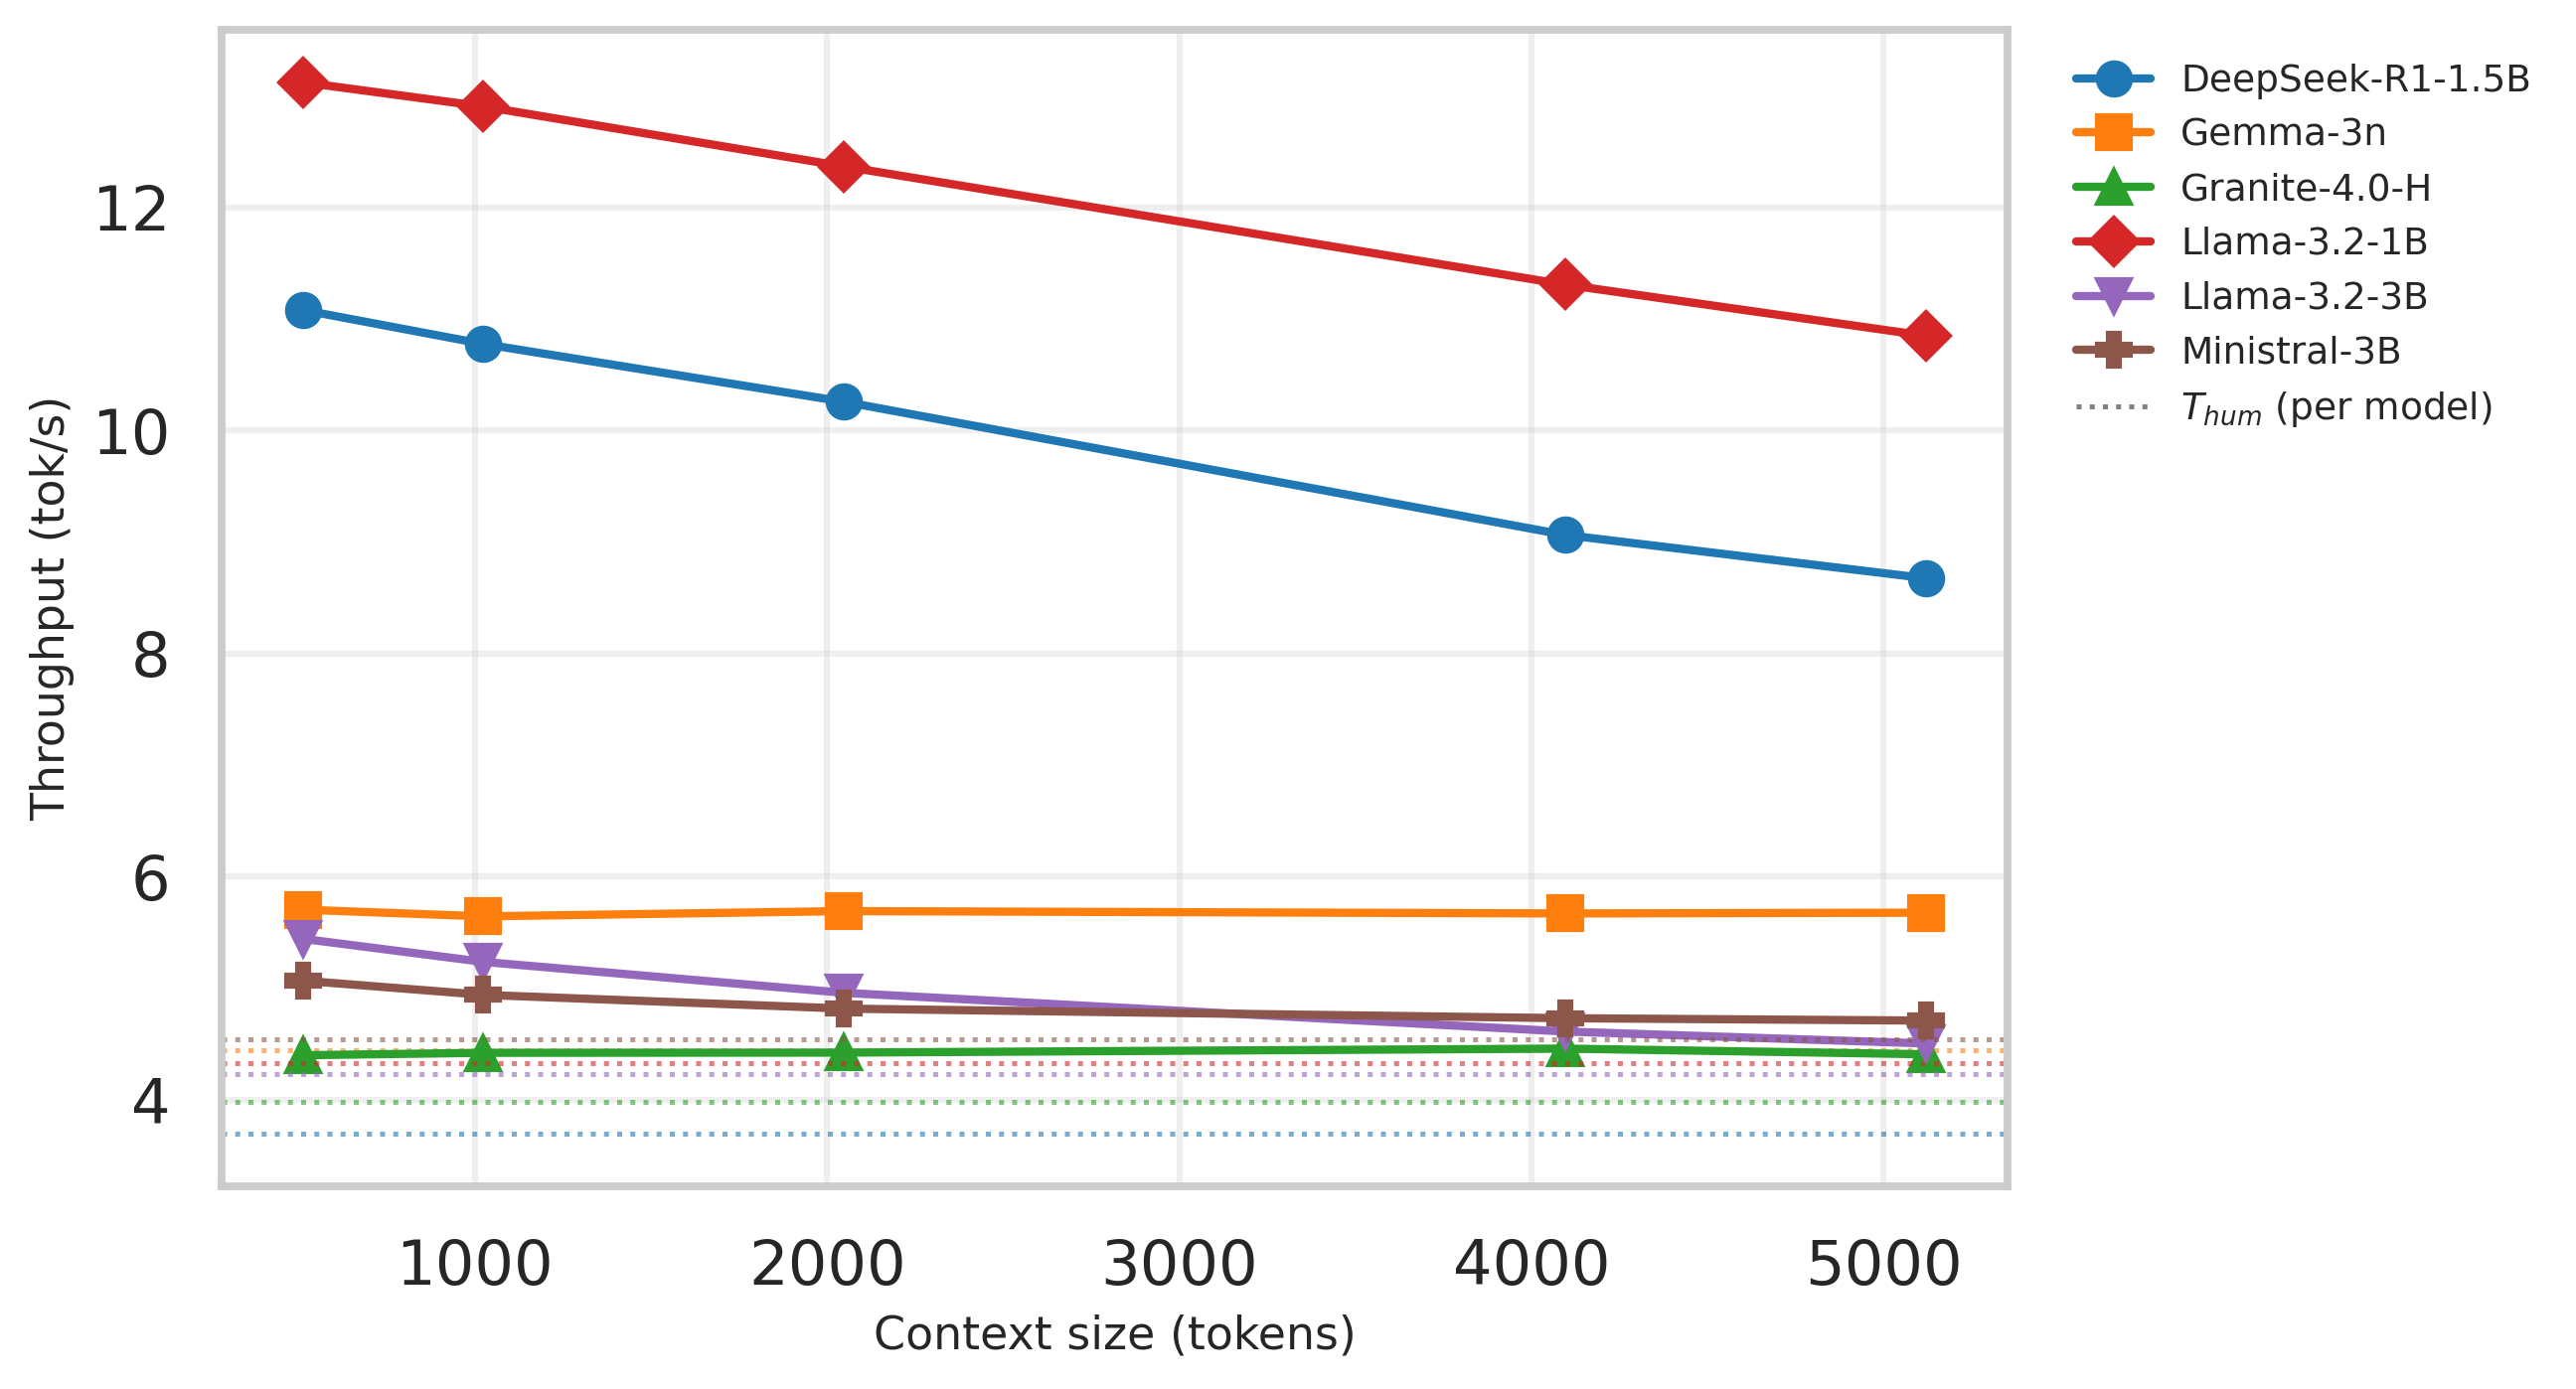
\includegraphics[width=\linewidth]{figures/e2_throughput.png}
\caption{Throughput (tok/s) versus context-window size, one line per model.
Dotted horizontal lines mark each model's usability threshold
$T_{\mathrm{hum}}$; every model stays above its threshold across the whole
range, so all configurations of the series remain usable. Active cooling.}
\label{fig:e2_throughput}
\end{figure}

\subsection{E3: Prefill Batch Size}\label{sec:results_e3}

in series E3, we varied the prefill batch size across 128--2\,048 (RQ3). The result
is itself a finding: the parameter has no appreciable effect on any
metric---RAM, throughput, TTFT, energy per token, and FoM remain constant
within experimental noise across the whole range, refuting the working
hypothesis that larger batches would raise throughput by exploiting the four
cores. The explanation is direct: in single-stream conversational inference
there are no concurrent requests to group, so prefill batching finds no
additional parallelism to exploit; the prefill of a single prompt already
saturates the available resources. The parameter can be left at its default
without penalty; any benefit could only emerge in concurrent deployments,
which are outside the scope of this study.

\subsection{E4: Inference Engine}\label{sec:results_e4}

in series E4, we compared llama.cpp and Ollama running the same models in identical
configurations, isolating the overhead of the runtime layer (RQ4).
Table~\ref{tab:e4} reports the results.

\begin{table}[!t]
\centering
\caption{llama.cpp (l.cpp) versus Ollama per model, with active cooling.
Positive $\Delta$ values indicate an Ollama advantage. \emph{Us.} marks the
usability of each engine's run (l.cpp/Ollama) against the corresponding
per-engine threshold $T_{\mathrm{hum}}$, computed empirically from the text
each engine generated. $^{\ddag}$~the Ollama run of DeepSeek-R1-1.5B is
non-usable because its anomalously high tokens-per-word ratio raises its
threshold to 13.76~tok/s, above the achieved throughput.}
\label{tab:e4}
\renewcommand{\arraystretch}{1.1}
\setlength{\tabcolsep}{2.6pt}
\footnotesize
\begin{tabular}{l r r c r r r r r r r r c}
\toprule
& \multicolumn{2}{c}{\textbf{$T$ (tok/s)}} & \textbf{$T_{\mathrm{hum}}$} &
\multicolumn{2}{c}{\textbf{TTFT (ms)}} &
\multicolumn{2}{c}{\textbf{$\varepsilon$ (tok/J)}} & \multicolumn{2}{c}{\textbf{FoM}} &
\textbf{$\Delta$\%} & \textbf{$\Delta$\%} & \textbf{Us.} \\
\cmidrule(lr){2-3}\cmidrule(lr){5-6}\cmidrule(lr){7-8}\cmidrule(lr){9-10}
\textbf{Model} & l.cpp & Oll. & \textbf{l.cpp/Oll.} & l.cpp & Oll. & l.cpp & Oll. & l.cpp & Oll. &
\textbf{$T$} & \textbf{FoM} & \textbf{l.cpp/Oll.} \\
\midrule
DeepSeek-R1-1.5B & 8.98  & 9.49 & 3.69/13.76 & 951  & 3111  & 1.251 & 1.337 & 1.025 & 1.035 & $+5.7$  & $+1.0$  & \ding{51}/\ding{55}$^{\ddag}$ \\
Llama-3.2-1B     & 11.23 & 11.16& 4.42/4.11 & 673  & 2552  & 1.733 & 1.623 & 0.961 & 0.906 & $-0.6$  & $-5.7$  & \ding{51}/\ding{51} \\
Llama-3.2-3B     & 4.61  & 5.08 & 4.25/4.22 & 1941 & 6563  & 0.681 & 0.669 & 1.000 & 1.030 & $+10.3$ & $+3.0$  & \ding{51}/\ding{51} \\
Gemma-3n         & 5.68  & 5.54 & 4.45/4.44 & 2613 & 7236  & 0.824 & 0.797 & 0.818 & 0.751 & $-2.5$  & $-8.2$  & \ding{51}/\ding{51} \\
Granite-4.0-H    & 4.41  & 4.32 & 3.99/3.92 & 2348 & 9932  & 0.658 & 0.592 & 0.934 & 0.883 & $-2.0$  & $-5.4$  & \ding{51}/\ding{51} \\
Ministral-3B     & 4.73  & 3.55 & 4.52/4.57 & 1929 & 12848 & 0.694 & 0.497 & 1.058 & 0.826 & $-25.0$ & $-21.9$ & \ding{51}/\ding{55} \\
\bottomrule
\end{tabular}
\end{table}

Decoding throughput is comparable between engines and shows no uniform
pattern (Ollama gains in two models, up to $+10.3\%$ in Llama-3.2-3B, and
loses in four, with a severe $-25\%$ penalty in Ministral-3B). The decisive
difference concentrates in TTFT: Ollama introduces a per-request
initialization overhead that multiplies first-token latency in every model,
exceeding a factor of six in the worst case (Ministral-3B: 12\,848~ms versus
1\,929~ms). Hardware utilization during generation
($\mathrm{MBU}_{\mathrm{corr}}$, $\eta_{\mathrm{CPU}}$) is similar between
engines, indicating that the difference stems not from the shared inference
core but from the orchestration layer~\cite{Github_Issue_Ollama}. A notable
exception is Gemma~3n's RAM footprint, which nearly doubles under Ollama
(4.30~GByte versus 2.16~GByte), suggesting less efficient memory management for its
MatFormer architecture. In usability terms, 10 of the 12 runs are usable and
the two non-usable runs both correspond to Ollama
(Table~\ref{tab:e4}): Ministral-3B falls below the threshold on raw
throughput (3.55~tok/s $< T_{\mathrm{hum}}$), and DeepSeek-R1-1.5B loses
usability because its Ollama run exhibits an anomalously high
tokens-per-word ratio that raises its threshold to
$T_{\mathrm{hum}}=13.76$~tok/s, above the achieved throughput. The
recommendation is to deploy llama.cpp
whenever response latency is a requirement, reserving Ollama for scenarios
where operational convenience outweighs immediacy.

\subsection{E5: Hailo-10H Accelerator}\label{sec:results_e5}

Finally, in series E5 we evaluated the Hailo-10H accelerator---contained in the
Raspberry~Pi AI~HAT+~2 add-on board attached to the platform for this
series---against CPU execution, running the entire model on the accelerator
through hailo-ollama (RQ5). The Hailo
backend does not report on inference phases, memory bandwidth, or token
probabilities; thus, for evaluation we used the reduced FoM defined in
Eq.~\eqref{eq:fom_red}. Unlike series E0--E4, energy was read from an
external wall-power meter for \emph{both} substrates, capturing HAT and
power-supply consumption; the reading includes boot and ${\sim}5$~minutes of
idle period before inference, so the resulting $\varepsilon$ values are lower
bounds, comparable within the series but not with E0--E4. Only the two models distributed by Hailo in
precompiled HEF format could be evaluated (DeepSeek-R1-1.5B and
Llama-3.2-3B). Table~\ref{tab:e5} reports the comparison.

\begin{table}[!t]
\centering
\caption{Hailo-10H versus CPU (llama.cpp) per model. Throughput (tok/s) and
energy efficiency $\varepsilon$ (tok/J) on both substrates, normalized factors
$T_{\mathrm{norm}}$ and $\varepsilon_{\mathrm{norm}}$, reduced FoM 
(Eq.~\eqref{eq:fom_red}), per-substrate usability threshold
$T_{\mathrm{hum}}$ computed empirically from this series' generated text, and
usability on each substrate (CPU/Hailo). $^{(1)}$~$\varepsilon$ derived from the external wall meter, whose reading
includes boot and ${\sim}5$\,min idle: lower bound, comparable between
substrates but not with series E0--E4.}
\label{tab:e5}
\renewcommand{\arraystretch}{1.1}
\setlength{\tabcolsep}{5pt}
\footnotesize
\begin{tabular}{l r r r r r r r r c c}
\toprule
& \multicolumn{2}{c}{\textbf{$T$ (tok/s)}} & \multicolumn{2}{c}{\textbf{$T_{\mathrm{hum}}$ (tok/s)}} &
\multicolumn{2}{c}{\textbf{$\varepsilon$ (tok/J)}$^{(1)}$} &
\textbf{$T_{\mathrm{norm}}$} & \textbf{$\varepsilon_{\mathrm{norm}}$} &
\textbf{FoM\textsubscript{red}} & \textbf{Us.} \\
\cmidrule(lr){2-3}\cmidrule(lr){4-5}\cmidrule(lr){6-7}
\textbf{Model} & CPU & Hailo & CPU & Hailo & CPU & Hailo & & & & C/H \\
\midrule
DeepSeek-R1-1.5B & 10.25 & 6.78 & 3.68 & 3.76 & 0.878 & 0.898 & 0.662 & 1.023 & 0.822 & \ding{51}/\ding{51} \\
Llama-3.2-3B     & 5.03  & 2.65 & 4.21 & 4.14 & 0.406 & 0.942 & 0.528 & 2.320 & 1.107 & \ding{51}/\ding{55} \\
\bottomrule
\end{tabular}
\end{table}

The results refute the expectation of acceleration: the Hailo-10H
\emph{reduces} throughput in both models, by 34\% in DeepSeek-R1-1.5B and
47\% in Llama-3.2-3B. The energy dimension, however, differs qualitatively
between models. For DeepSeek-R1-1.5B the accelerator offers no appreciable
energy advantage ($\varepsilon_{\mathrm{norm}}=1.023$), so the CPU dominates
on both axes ($\mathrm{FoM}_{\mathrm{red}}=0.822$). For Llama-3.2-3B the
energy gain is notable---57\% lower cost per token
($\varepsilon_{\mathrm{norm}}=2.320$)---which more than compensates the speed
loss and raises $\mathrm{FoM}_{\mathrm{red}}$ to 1.107, above parity with the
CPU. Usability disqualifies this advantage: Llama-3.2-3B, usable on CPU, falls
below $T_{\mathrm{hum}}$ on the accelerator. The result must also be read in
the context of the maturity of the generative-inference software stack for
Hailo, considerably less optimized than the CPU stack. In its current state,
the Hailo-10H is therefore \emph{not} recommended for the general case: it is
advisable only under strict energy constraints, provided that the integrator can
accept the loss of speed and interactivity, the limitations
of the accelerator---above all the restricted catalog of precompiled HEF
models and the context/batch parameters fixed at compilation time---and
models of sufficient size (Llama-3.2-3B or larger) for the efficiency
advantage to compensate the speed penalty.

\subsection{Synthesis}\label{sec:synthesis}

The results from the six series converge on a coherent picture articulated around the three
transversal axes elaborated next. 

\paragraph{Memory bandwidth is the dominant limiting factor.}
The target platform operates memory-bound during decoding, with
$\mathrm{MBU}_{\mathrm{corr}}$ between 50 and 72\% in nominal conditions.
This single bottleneck explains four series: in E1, stronger quantization
relieves memory traffic and raises throughput monotonically down to
${\approx}4$~bits; in E2, larger context windows increase KV-cache traffic
and degrade throughput by up to 22\% in the models most dependent on MBU; in
E3, prefill batch size is irrelevant because single-stream decoding finds no
additional parallelism; and in E4, llama.cpp's serverless architecture
reduces first-token latency without altering decoding throughput.

\paragraph{A well-defined optimal reference configuration.}
Active cooling, Q4\_K\_M quantization, and the llama.cpp engine constitute
the recommended configuration for interactive deployments: it keeps all six
models usable, minimizes TTFT, and offers the best balance between
throughput, memory footprint, and energy cost, while degrading perplexity by
less than 5\% with respect to Q8\_0. Q4\_0 and Q3\_K\_M can substitute
Q4\_K\_M under severe resource constraints, with the caveat that Q4\_0 shows
higher quality degradation at the same bit level.

\paragraph{Hardware acceleration introduces an asymmetric, model-dependent
balance.}
The Hailo-10H does not improve throughput---it reduces it by 34--47\%---but
provides a substantial energy advantage for sufficiently large models,
lifting Llama-3.2-3B above CPU parity
($\mathrm{FoM}_{\mathrm{red}}=1.107$) through a 57\% reduction in energy per
token. Hardware acceleration can pay off in energy-constrained scenarios
with medium-size models, but it does not replace the CPU in the general
case: the speed and interactivity loss, the immature software ecosystem, and
the platform's own restrictions---a catalog limited to the precompiled HEF
models distributed by the vendor, with context and batch fixed at
compilation time---currently outweigh the energy advantage outside that
niche.

Overall, the results obtained in this study answer the seven research questions initially posed
and confirm that the Raspberry~Pi~5 is a viable platform for local, interactive SLM inference
with the appropriate configuration and within the size and quantization
limits identified in this work.

% =====================================================================
\section{Conclusions}\label{sec:conclusions}
% =====================================================================

We have presented a systematic analysis and optimization of SLM 
inference on the Raspberry~Pi~5, evaluating the impact of six
experimental factors---cooling, quantization, context size, prefill batch,
inference engine, and hardware acceleration---on performance, energy
efficiency, and interactive usability, supported by two reusable open-source
tools (\textit{MonitorSystem} and \textit{monitorviz}) that jointly close the instrumentation
gap identified in the literature.

The main conclusions are: (i)~active cooling is an enabling requirement, not
an optimization---without it, thermal throttling collapses compute
efficiency from ${\approx}0.97$ to ${\approx}0.40$ and renders four of six
models non-interactive; (ii)~4-bit quantization is the optimum on this
memory-bound platform, with Q4\_K\_M as the best default operating point in
both performance and quality, whereas 8-bit and full-precision formats are
counterproductive; (iii)~context size is a fine-tuning parameter (throughput
losses up to 22\%) and prefill batch size is irrelevant in single-stream
inference; (iv)~llama.cpp is the preferable engine when latency matters,
with up to $6\times$ lower TTFT than Ollama at comparable decoding
throughput; (v)~the Hailo-10H accelerator trades throughput for energy and is
not recommended in the general case---only under energy constraints, with
sufficiently large models, and accepting the loss of interactivity and the
platform's restrictions on available models;
(vi)~decoding concentrates virtually the entire temporal and energy cost,
with model loading negligible in steady operation; and (vii)~a unified,
reproducible measurement framework integrating temporal, energy, and thermal
metrics is feasible on this class of platform.

\paragraph{Limitations.}
All experiments targeted a single platform (Raspberry~Pi~5); results do not
transfer directly to other edge devices with different memory bandwidth and
thermal envelopes. The internal power sensor in series E0--E4 excludes the
cooler and peripherals (lower bounds), and its measurement protocol differs
from the external meter of E5, precluding absolute cross-series energy
comparisons. Series E5 is restricted to the two models distributed in
precompiled HEF format, with context and batch fixed at compilation time.
All experiments were single-stream; conclusions on batching (E3) and engines
(E4) do not extend to concurrent deployments. Quality evaluation is limited
to perplexity, which is not comparable across tokenizers and does not
capture task suitability; only post-training GGUF quantization was evaluated
among compression techniques; and the study covers text-only models with a
general-purpose prompt set.

\paragraph{Future work.}
Natural extensions include 1) broadening the model set (0.5--8B, mixtures of
experts, recurrent-state and multimodal models) and the accelerator series
once user-compilable HEF flows become available; 2) extending \textit{MonitorSystem} and
\textit{monitorviz} to multimodal workloads and additional platforms (e.g., Jetson
Orin Nano); 3) evaluating further compression and adaptation techniques
(pruning, distillation, LoRA-based fine-tuning) under the same metric
framework; 4) studying concurrent multi-stream deployments and tool-calling
integration with edge monitoring systems; and 5) building a domain-specific
biodiversity corpus and functional evaluation suite to complete the
framework with an application-oriented quality layer.

%% Acknowledgments — TODO: add funding/collaboration acknowledgments
%% (e.g., collaboration grant, research group) before submission.
%\begin{acks}
%\end{acks}

\printbibliography

\end{document}
